\documentclass[11pt,a4paper]{report}
% Packages for formatting, math, and graphics
\usepackage{times}
\usepackage[pdftex]{graphicx}
\usepackage{amsmath}
\usepackage{longtable}
\usepackage[acronym]{glossaries}  % Changed from acronym to glossaries
\usepackage[utf8]{inputenc}
\usepackage{color}
\usepackage{amssymb}
\usepackage{caption}
\usepackage{subcaption}
\usepackage{txfonts}
\usepackage{mathdots}
\usepackage{rotating}
\usepackage{array}
\usepackage[classicReIm]{kpfonts}
% Graphics file extensions
\DeclareGraphicsExtensions{.pdf,.jpeg,.png,.PNG}
% Hyperref setup for links
\usepackage{hyperref}
\hypersetup{
    colorlinks=true,
    linkcolor=blue,
    filecolor=magenta,      
    urlcolor=cyan,
    citecolor=red
}
\urlstyle{same}
% Additional packages for math, citations, and layout
\usepackage{mathtools}
\usepackage[numbers,sort&compress]{natbib}  % Changed from [superscript]{cite}
\usepackage[top=2cm, bottom=2cm, left=2.5cm, right=2cm]{geometry}
\usepackage[compact]{titlesec}
\usepackage{fancyhdr}
\usepackage{setspace}
\usepackage[T1]{fontenc}  % Changed to [T1]
\usepackage{microtype}
\usepackage{booktabs}
\usepackage{multirow}
\usepackage[table,xcdraw]{xcolor}
\usepackage[printwatermark]{xwatermark}
\usepackage{transparent}
\usepackage{algorithm2e}
\usepackage{algorithm}
\usepackage[noend]{algpseudocode}
\usepackage[final]{pdfpages}
\usepackage{MnSymbol,wasysym}
% Document settings
\tolerance=1
\emergencystretch=\maxdimen
\hyphenpenalty=10000
\hbadness=10000
\setlength{\arrayrulewidth}{0.4mm}
\setlength{\tabcolsep}{18pt}
\renewcommand{\arraystretch}{1.5}
% Page style settings
\pagestyle{fancy}
\fancyhf{} 
\fancyhead[R]{\itshape\leftmark}
\fancyfoot[C]{\thepage}
\renewcommand\headrulewidth{0pt}
% URL hyphenation
\PassOptionsToPackage{hyphens}{url}
% Font and spacing
\usepackage{mathptmx}
\linespread{1.5}
% Load glossaries
\makeglossaries

% Load abbreviations
% Acronym definitions
\newacronym{AI}{AI}{Artificial Intelligence}
\newacronym{ML}{ML}{Machine Learning}
\newacronym{DL}{DL}{Deep Learning}
\newacronym{NLP}{NLP}{Natural Language Processing}
\newacronym{CV}{CV}{Computer Vision}
\newacronym{eBPF}{eBPF}{extended Berkeley Packet Filter}
\newacronym{OCSF}{OCSF}{Open Cybersecurity Schema Framework}
\newacronym{SIEM}{SIEM}{Security Information and Event Management}
\newacronym{IoT}{IoT}{Internet of Things}
\newacronym{API}{API}{Application Programming Interface}
\newacronym{JSON}{JSON}{JavaScript Object Notation}
\newacronym{HTTP}{HTTP}{Hypertext Transfer Protocol}
\newacronym{HTTPS}{HTTPS}{Hypertext Transfer Protocol Secure}
\newacronym{TCP}{TCP}{Transmission Control Protocol}
\newacronym{UDP}{UDP}{User Datagram Protocol}
\newacronym{IP}{IP}{Internet Protocol}
\newacronym{DNS}{DNS}{Domain Name System}
\newacronym{SQL}{SQL}{Structured Query Language}
\newacronym{NoSQL}{NoSQL}{Not Only SQL}
\newacronym{XSS}{XSS}{Cross-Site Scripting}

\begin{document}
% Front matter
\renewcommand{\thepage}{\roman{page}}
% TITLE PAGE
\thispagestyle{empty}
%\addcontentsline{toc}{chapter}{Cover Page}\index{Cover Page}
\begin{center}
\setstretch{2}
\textcolor{purple}{{\huge \textsc{OpenArmor: Smarter Cybersecurity powered by advanced logging} }}\\
\vspace{0.5cm}
A Project Report
Submitted By\\

\textcolor{olive}{\huge \bf ANUBHAV GAIN-210303126225}\\ 
\textcolor{olive}{\huge \bf HRIDAY SHETH-210303124120}\\  
\textcolor{olive}{\huge \bf SHARADA CHIPLUNKAR-210303126223}\\ 
\textcolor{olive}{\huge \bf PRIYANSHU BHANA-210303126222}\\ 

\vspace{0.4cm}
in Partial Fulfilment For the Award of
the Degree of\\
BACHELOR OF TECHNOLOGY
COMPUTER SCIENCE \& ENGINEERING\\
Under the Guidance of\\
\large{\textbf{Prof. Ishan K Rajani}}\\
Assistant Professor, \\
CSE
PIET,  Parul University \\
\large{\textbf{Prof. Avnish Jani}}\\
Assistant Professor, \\
CSE
PIET,  Parul University \\

\vspace{0.3cm}
\begin{figure}[h]
\begin{center}
     
\includegraphics[scale=0.18]{parullogo.png} \\
     \vspace{0.7cm}
     \includegraphics[scale=0.02]{Digital Use - PU NAAC Logo.jpg}
\end{center}
\end{figure}
%\textcolor{teal}{\textbf{\Huge{PARUL UNIVERSITY \\ %\textbf{NAAC A++}}}}\\
VADODARA\\
April - 2024
\end{center}

\thispagestyle{plain}
\setstretch{1.5}
%\fontfamily{qag}\selectfont
\begin{figure}
    \centering
    
\includegraphics[scale=0.15]{parullogo.png}
\end{figure}
\vspace{1.5cm}
\begin{center}
    {\Huge \textsc{\color{violet}PARUL UNIVERSITY}}\\
   
    \vspace{1cm}
     {\Huge \bf \textsc{\color{teal}Certificate}}\\
     \vspace{0.5cm}
\end{center}
\large{This is to Certify that Project - 1 (203105499) of 6$^{th}$ Semester entitled "OpenArmor: Smarter Cybersecurity Powered by Advanced Logging" of Group No. PUCSE\_328 has been successfully completed by}
\begin{itemize}
\centering
    \item ANUBHAV GAIN - 210303126225
    \item HRIDAY SHETH - 210303124120
    \item SHARADA CHIPLUNKAR - 210303126223
    \item PRIYANSHU BHANA - 210303126222
\end{itemize}
     
\noindent
\large{under my guidance in partial fulfillment of the Bachelor of Technology (B.Tech) in Computer Science \& Engineering of Parul University in Academic Year 2023-2024.}\\
\par
\vspace{0.5cm}
Date of Submission: \_\_\_\_\_\_\_\_\_\_\_\_\_\_\_\_\_\_

\vspace{2.5cm}
\begin{tabular}{l r r}
\color{brown}
  \textbf{Prof. Ishan K. Rajani}, & \hspace{1cm}
  \color{brown}\textbf{Prof. Avnish Jani}, & \hspace{1cm}
  \color{brown}\textbf{Dr. Amit Barve,}  \\ 
  Project Guide & Project Guide & Head of Department,  \\ 
  Project Coordinator:- & & CSE, PIET \\
  Parul University  & & \\ [7ex]  
  %& External Examiner 
\end{tabular}
% ACKNOWLEDGEMENT PAGE
\thispagestyle{empty}
\newpage
\cleardoublepage\phantomsection
\addcontentsline{toc}{chapter}{Acknowledgements}\index{Acknowledgements}
\begin{center}
{\Large \bf Acknowledgements}\\
\end{center}
\vspace{10pt}

\begin{flushright}
\textit{"The single greatest cause of happiness is gratitude."}\\
\vspace{5mm}
— Auliq-Ice
\end{flushright}

The completion of this project would not have been possible without the help and support of many individuals and institutions. 

First, we sincerely thank our project guide, \textbf{Professor Ishan K. Rajani}, for his expert guidance, continuous encouragement, and unwavering support throughout the project. His patience, advice, and willingness to share knowledge were invaluable in shaping our work and overcoming various challenges. 

We also extend our heartfelt gratitude to the \textbf{CSE Department}, especially \textbf{Dr. Kruti Sutaria} and \textbf{Professor Yatin Shukla}, for their valuable feedback, insightful inputs, and assistance at various stages of the project. Their expertise significantly enriched our understanding.

Additionally, we are deeply grateful to the open-source community and the developers behind the technologies we utilized, such as \textbf{eBPF}, \textbf{OCSF}, and various AI/ML libraries. Their contributions were instrumental in facilitating our research and advancing cybersecurity innovation.

We would also like to thank our fellow students, whose time, efforts, and ideas greatly enhanced our group discussions and collaborations. Their diverse perspectives helped us refine and improve our work.

Finally, we owe profound gratitude to our families and friends for their unconditional love, encouragement, and motivation throughout this journey. Their belief in us provided the strength we needed to overcome challenges and persevere. 

This project would not have been possible without the collective efforts and contributions of all these individuals and institutions. We deeply appreciate their invaluable support.

\vspace{1.5cm}
\begin{flushright}
\textbf{Anubhav Gain (210303126225)}\\
\textbf{Hriday Sheth (210303124120)}\\
\textbf{Sharada Chiplunkar (210303126223)}\\
\textbf{Priyanshu Bhana (210303126222)}\\
CSE Department, PIET\\
Parul University,\\
Vadodara
\end{flushright}

\thispagestyle{empty}
\newpage
\cleardoublepage\phantomsection
\addcontentsline{toc}{chapter}{Abstract}\index{Abstract}
\begin{center}
{\Large \bf Abstract}\\
\end{center}
\vspace{10pt}

\textbf{OpenArmor: Intelligent Cybersecurity Powered by Advanced Logging}

In today’s digital landscape, the rise of sophisticated cyber threats compels organizations to adopt stronger defenses. However, traditional security measures often struggle to keep up with the dynamic nature and complexity of modern attacks. To address these challenges, we introduce \textbf{OpenArmor}—an innovative cybersecurity solution that integrates advanced logging techniques with state-of-the-art artificial intelligence (AI) and machine learning (ML). This powerful combination enables proactive threat detection, automated analysis, and rapid response capabilities.

At its core, OpenArmor leverages the \textbf{extended Berkeley Packet Filter (eBPF)}, a cutting-edge kernel-level technology that allows efficient and comprehensive system activity logging. By extracting data directly from the Linux kernel, OpenArmor offers unparalleled visibility into system operations, capturing granular insights often overlooked by traditional logging methods. These detailed logs provide the foundation for OpenArmor’s advanced security analytics.

To ensure seamless integration with existing security infrastructures, OpenArmor structures its logs according to the \textbf{Open Cybersecurity Schema Framework (OCSF)}, a widely adopted industry standard. This compatibility allows OpenArmor to interface smoothly with security information and event management (SIEM) platforms, enabling organizations to maximize the value of their existing security tools while gaining enhanced threat detection capabilities.

The true strength of OpenArmor lies in its \textbf{AI- and ML-powered analytics}. Through advanced algorithms, the system establishes a dynamic baseline of normal system behavior, allowing it to detect even subtle anomalies that may indicate potential threats. This proactive detection ensures organizations stay ahead of attacks rather than reacting to them after the fact.

OpenArmor continuously monitors system activity, using AI to correlate events and recognize patterns indicative of security incidents. By automating these processes, it significantly reduces the burden on security teams, enabling them to focus on high-priority tasks while ensuring no potential threat goes undetected.

\newpage
Additionally, OpenArmor provides \textbf{intelligent alerts} with actionable insights, empowering security professionals to respond swiftly and effectively. These alerts are tailored to the specific needs of the organization, taking into account factors such as industry regulations, compliance requirements, and risk profiles. This ensures responses are efficient, targeted, and context-aware.

By combining advanced logging with AI and ML capabilities, OpenArmor offers a comprehensive, adaptive cybersecurity solution that continuously monitors, analyzes, and evolves with emerging threats. Its proactive threat detection, automated analysis, and contextual alerting system represent a paradigm shift in cybersecurity, reducing risk exposure and strengthening defenses.

OpenArmor marks the beginning of a new era in \textbf{intelligent cybersecurity}, enabling organizations to stay ahead of evolving threats. By leveraging the synergy between advanced logging and AI-powered analytics, OpenArmor provides a robust, adaptive security posture—protecting critical systems and data while allowing organizations to focus confidently on their core operations.

% Table of Contents
\cleardoublepage
\phantomsection
\renewcommand{\contentsname}{Table of Contents}
\addcontentsline{toc}{chapter}{\contentsname}
\tableofcontents

% List of Abbreviations
% This section is now handled in the main.tex file

% List of Symbols
\cleardoublepage
\phantomsection
\addcontentsline{toc}{chapter}{List of Symbols}
\chapter*{List of Symbols}
\begin{tabular}{@{}lp{0.8\textwidth}}
    $\alpha$ & Alpha (used for significance level in statistical tests) \\
    $\beta$ & Beta (used for type II error probability) \\
    $\gamma$ & Gamma (often used for the Euler-Mascheroni constant) \\
    $\delta$ & Delta (used to denote change or difference) \\
    $\epsilon$ & Epsilon (often used to denote a small positive quantity) \\
    $\zeta$ & Zeta (used in the Riemann zeta function) \\
    $\eta$ & Eta (often used for efficiency in physics) \\
    $\theta$ & Theta (often used for angles) \\
    $\lambda$ & Lambda (used in various contexts, including eigenvalues) \\
    $\mu$ & Mu (used for population mean) \\
    $\pi$ & Pi (ratio of a circle's circumference to its diameter) \\
    $\rho$ & Rho (often used for density or correlation coefficient) \\
    $\sigma$ & Sigma (used for standard deviation) \\
    $\tau$ & Tau (often used as an alternative to pi in some contexts) \\
    $\phi$ & Phi (often used for the golden ratio) \\
    $\chi$ & Chi (used in chi-squared distribution) \\
    $\psi$ & Psi (used in various contexts in physics and mathematics) \\
    $\omega$ & Omega (often used for angular velocity) \\
    $\exists$ & There exists
\end{tabular}

% List of Definitions
\cleardoublepage
\phantomsection
\addcontentsline{toc}{chapter}{List of Definitions}
\chapter*{List of Definitions}
\begin{description}
    \item[Artificial Intelligence] The simulation of human intelligence processes by machines, especially computer systems.
    \item[Machine Learning] A subset of AI that provides systems the ability to automatically learn and improve from experience without being explicitly programmed.
    \item[Deep Learning] A subset of machine learning based on artificial neural networks with representation learning.
    \item[Cybersecurity] The practice of protecting systems, networks, and programs from digital attacks.
    \item[Big Data] Extremely large data sets that may be analyzed computationally to reveal patterns, trends, and associations.
    \item[Cloud Computing] The delivery of computing services over the Internet ("the cloud") to offer faster innovation, flexible resources, and economies of scale.
    \item[Blockchain] A decentralized, distributed ledger technology that records the provenance of a digital asset.
    \item[Quantum Computing] A type of computation that harnesses the collective properties of quantum states, such as superposition, interference, and entanglement, to perform calculations.
    \item[Edge Computing] A distributed computing paradigm that brings computation and data storage closer to the location where it is needed.
    \item[5G] The fifth generation technology standard for broadband cellular networks.
\end{description}

\cleardoublepage
% Include the list of abbreviations
\cleardoublepage
\phantomsection
\addcontentsline{toc}{chapter}{List of Abbreviations}
\printglossary[type=\acronymtype,title={List of Abbreviations}]
% Main content
\pagenumbering{arabic}
\pagestyle{fancy}
\renewcommand{\chaptermark}[1]{\markboth{\chaptername \ \thechapter \ -\ #1}{}}
\renewcommand{\headrulewidth}{2pt}
\renewcommand{\footrulewidth}{1pt}
\chapter{Introduction}\doublespacing

\section{Background}
In the rapidly evolving digital landscape of the 21st century, cybersecurity has become a critical concern for organizations across all sectors. The frequency, sophistication, and impact of cyber attacks are increasing at an alarming rate, posing significant risks to data integrity, operational continuity, and organizational reputation. Traditional security measures, while still necessary, are often insufficient to combat the complex and dynamic nature of modern cyber threats. This pressing need for more advanced, intelligent, and proactive cybersecurity solutions has led to the development of OpenArmor.

\section{Introduction to OpenArmor}
OpenArmor is an innovative cybersecurity solution designed to address the challenges posed by the ever-evolving threat landscape. By leveraging advanced logging techniques, artificial intelligence (AI), and machine learning (ML) algorithms, OpenArmor provides a comprehensive and proactive approach to threat detection, analysis, and response. This cutting-edge system aims to revolutionize the way organizations protect their digital assets and maintain their security posture in an increasingly hostile cyber environment.

\section{Purpose of the Document}
This project report serves as a comprehensive guide to OpenArmor, detailing its objectives, scope, and technical specifications. The document aims to:

\begin{itemize}
    \item Provide a clear overview of OpenArmor's core functionalities and innovative features
    \item Explain the advanced logging system and its integration with AI/ML capabilities
    \item Detail the proactive threat detection and alert mechanisms
    \item Offer insights into the development, implementation, and deployment processes of OpenArmor
    \item Serve as a reference for all stakeholders involved in the project
\end{itemize}

By offering a thorough understanding of OpenArmor, this document facilitates effective communication, collaboration, and decision-making throughout the project lifecycle.

\section{Document Conventions}
To ensure clarity and consistency, this document adheres to the following conventions:

\begin{itemize}
    \item Clear and concise language is used throughout to enhance readability
    \item Technical terms are defined upon first use and included in a glossary
    \item Requirements are categorized and prioritized using the MoSCoW method (Must have, Should have, Could have, Won't have)
    \item Diagrams and flowcharts are used to illustrate complex concepts and processes
    \item Each section begins with a brief overview of its contents
\end{itemize}

These conventions are designed to make the document accessible to all stakeholders, regardless of their technical background.

\section{Intended Audience}
This document is intended for a diverse audience, including:

\begin{itemize}
    \item Software Developers: To understand the technical requirements and system architecture
    \item Cybersecurity Experts: To gain insights into the advanced threat detection mechanisms
    \item Project Managers: To oversee the development process and resource allocation
    \item System Administrators: To understand deployment and integration requirements
    \item Business Stakeholders: To comprehend the value proposition and potential impact of OpenArmor
\end{itemize}

Readers are encouraged to focus on sections most relevant to their roles, using the table of contents as a guide.

\section{Product Scope}
OpenArmor is a comprehensive cybersecurity solution designed to:

\begin{itemize}
    \item Utilize extended Berkeley Packet Filter (eBPF) technology for advanced system activity logging
    \item Employ AI and ML algorithms for real-time threat detection and analysis
    \item Provide a user-friendly interface for monitoring system activity and security alerts
    \item Integrate seamlessly with existing security information and event management (SIEM) systems
    \item Offer customizable alert mechanisms and response protocols
    \item Ensure compliance with industry standards and regulations
    \item Adapt to emerging threats through continuous learning and updates
\end{itemize}

By offering these features, OpenArmor aims to significantly enhance an organization's ability to detect, prevent, and respond to cyber threats, thereby reducing overall risk exposure and ensuring operational resilience in the face of evolving cyber challenges.
\chapter{Literature Survey}

\section{Introduction}
This chapter presents a comprehensive review of recent research relevant to the development of OpenArmor. The survey covers various aspects of cybersecurity, including eBPF technology, AI-driven security solutions, event extraction, monitoring systems, and semantic web approaches for cybersecurity information management. Each paper is summarized and its relevance to OpenArmor is discussed.

\section{Advanced Network Functions and Monitoring}
\subsection{eBPF-Based Network Functions}
\textbf{Title}: A Framework for eBPF-Based Network Functions in an Era of Microservices 
\textbf{Authors}: Miano, S., Risso, F., Bernal, M. V., Bertrone, M., and Lu, Y. (2021)
\textbf{Publication}: IEEE Transactions on Network and Service Management, 18(1), 133-151

\textbf{Summary}: [Your existing summary]

\textbf{Relevance to OpenArmor}: This paper's framework for eBPF-based network functions aligns closely with OpenArmor's use of eBPF for advanced system activity logging. The high performance and flexibility demonstrated in this research validate the choice of eBPF technology for OpenArmor's core logging functionality.

\subsection{Distributed Cloud Monitoring}
\textbf{Title}: Distributed cloud monitoring using Docker as next generation container virtualization technology
\textbf{Authors}: Dhakate, S., and Godbole, A. (2015)
\textbf{Publication}: 2015 Annual IEEE India Conference (INDICON) (pp. 1-5)

\textbf{Summary}: [Your existing summary]

\textbf{Relevance to OpenArmor}: The distributed monitoring approach using containerization technology could inform OpenArmor's architecture, especially for deploying and managing monitoring components across diverse environments.

\section{AI and Machine Learning in Cybersecurity}
\subsection{AI-Driven Cybersecurity Overview}
\textbf{Title}: AI‑Driven Cybersecurity: An Overview, Security Intelligence Modeling and Research Directions
\textbf{Authors}: Sarker, I. H., Furhad, M. H., and Nowrozy, R. (2021)
\textbf{Publication}: SN Computer Science, 2(3), 173

\textbf{Summary}: [Your existing summary]

\textbf{Relevance to OpenArmor}: This paper provides a comprehensive overview of AI applications in cybersecurity, which is directly relevant to OpenArmor's AI-driven threat detection and analysis capabilities. The research directions outlined could guide future enhancements of OpenArmor.

\section{Cybersecurity Event Extraction and Analysis}
\subsection{Document-level Cybersecurity Event Extraction}
\textbf{Title}: A Framework for Document-level Cybersecurity Event Extraction from Open Source Data
\textbf{Authors}: Luo, N., Du, X., He, Y., Jiang, J., Wang, X., Jiang, Z., and Zhang, K. (2021)
\textbf{Publication}: 2021 IEEE 24th International Conference on Computer Supported Cooperative Work in Design (CSCWD) (pp. 422-427)

\textbf{Summary}: [Your existing summary]

\textbf{Relevance to OpenArmor}: The event extraction framework presented in this paper could enhance OpenArmor's ability to process and analyze unstructured data sources, improving threat intelligence capabilities.

\subsection{Rich Semantic Information Extraction}
\textbf{Title}: Extracting rich semantic information about cybersecurity events
\textbf{Authors}: Satyapanich, T., Finin, T., and Ferraro, F. (2019)
\textbf{Publication}: 2019 IEEE International Conference on Big Data (Big Data) (pp. 5034-5042)

\textbf{Summary}: [Your existing summary]

\textbf{Relevance to OpenArmor}: This research could inform the development of OpenArmor's data processing pipeline, enabling more comprehensive and semantically rich threat intelligence extraction from diverse data sources.


\section{Research Paper 1}
\textbf{Title }: A Framework for eBPF-Based Network Functions in an Era of Microservices 
\\
\textbf{Author }: Miano, S., Risso, F., Bernal, M. V., Bertrone, M., and Lu, Y. (2021). A framework for eBPF-based network functions in an era of microservices. IEEE Transactions on Network and Service Management, 18(1), 133-151.
\\
\textbf{Summary }: The paper proposes a framework that leverages eBPF (extended Berkeley Packet Filter) technology to develop and deploy network functions as eBPF programs in microservices environments. The framework consists of components for eBPF program development, deployment, and communication, enabling efficient and scalable implementation of network functions like load balancers and firewalls. Evaluation results demonstrate the framework's ability to achieve high throughput and low latency, comparable or better than traditional kernel-bypass solutions, while offering improved flexibility and agility in provisioning network functions.

\section{Research Paper 2}
\textbf{Title} : A Framework for Document-level Cybersecurity Event Extraction from Open Source Data
\\
\textbf{Author} : Luo, N., Du, X., He, Y., Jiang, J., Wang, X., Jiang, Z., and Zhang, K. (2021, May). A framework for document-level cybersecurity event extraction from open source data. In 2021 IEEE 24th International Conference on Computer Supported Cooperative Work in Design (CSCWD) (pp. 422-427). IEEE.
\\
\newpage
\textbf{Summary} : The paper presents a framework for extracting cybersecurity events from open-source data at the document level. It proposes a deep learning model that performs joint entity recognition and event extraction, capturing both intra- and inter-sentence dependencies. The framework leverages external knowledge bases to enrich the extracted events with contextual information. Experimental results on real-world datasets demonstrate the framework's effectiveness in accurately identifying and characterizing cybersecurity incidents from unstructured text data.

\section{Research Paper 3}
\textbf{Title }: Distributed cloud monitoring using Docker as next generation container virtualization technology
\\
\textbf{Author }: Dhakate, S., and Godbole, A. (2015, December). Distributed cloud monitoring using Docker as next generation container virtualization technology. In 2015 Annual IEEE India Conference (INDICON) (pp. 1-5). IEEE.
\\
\textbf{Summary }: This paper proposes a distributed cloud monitoring system that leverages Docker, a next-generation container virtualization technology. The system employs Docker containers to encapsulate monitoring agents, enabling efficient deployment and management of monitoring components across distributed cloud environments. The authors demonstrate the system's ability to monitor cloud resources effectively while minimizing overhead and providing scalability benefits compared to traditional virtualization approaches.

\section{Research Paper 4}
\textbf{Title} : AI‑Driven Cybersecurity: An Overview, Security Intelligence Modeling and Research Directions
\\
\textbf{Author} : Sarker, I. H., Furhad, M. H., and Nowrozy, R. (2021). Ai-driven cybersecurity: an overview, security intelligence modeling and research directions. SN Computer Science, 2(3), 173.
\\
\textbf{Summary} : This paper provides an overview of leveraging artificial intelligence (AI) for cybersecurity. It explores various AI and machine learning techniques like deep learning, reinforcement learning, and ensemble methods that can be applied to domains such as network security, malware detection, and intrusion prevention. The authors highlight the benefits of AI-driven security solutions, including adaptability, scalability, and proactive threat detection capabilities. The paper also outlines research challenges and future directions for developing robust AI-based cybersecurity systems, such as handling adversarial attacks, dealing with data scarcity, and ensuring model transparency and interpretability.

\section{Research Paper 5}
\textbf{Title} : Unpacking strategic behavior in cyberspace: a schema-driven approach
\\
\textbf{Author} : Gomez, M. A., and Whyte, C. (2022). Unpacking strategic behavior in cyberspace: a schema-driven approach. Journal of Cybersecurity, 8(1), tyac005.
\\
\textbf{Summary} : This paper proposes a schema-driven approach to analyze and understand strategic behavior in cyberspace. It introduces a framework that combines cognitive schemas and game theory to model the decision-making processes and interactions between adversaries in cyber conflicts. The authors argue that this approach can provide insights into the motivations, goals, and potential actions of cyber threat actors, enabling more effective cybersecurity strategies and deterrence mechanisms. The framework is illustrated through case studies, demonstrating its applicability in unpacking the complexities of strategic cyber behavior.

\section{Research Paper 6}
\textbf{Title} : Developing a UI and Automation Framework for a Cybersecurity Research and Experimentation Environment
\\
\textbf{Author} : Butler, C., Thompson, G., Hsieh, G., Hoppa, M. A., and Nauer, K. S. (2018). Developing a UI and Automation Framework for a Cybersecurity Research and Experimentation Environment. In Proceedings of the International Conference on Security and Management (SAM) (pp. 208-213). The Steering Committee of The World Congress in Computer Science, Computer Engineering and Applied Computing (WorldComp).
\\
\textbf{Summary} : The paper describes the development of a user interface (UI) and automation framework for a cybersecurity research and experimentation environment. The framework aims to simplify the process of configuring and deploying cybersecurity experiments, enabling researchers to focus on their core objectives. It provides a web-based UI for defining experiment parameters and orchestrating the deployment of virtual machines and network configurations. The automation capabilities streamline the setup, execution, and data collection phases of cybersecurity experiments, enhancing productivity and reproducibility.

\newpage
\section{Research Paper 7}
\textbf{Title} : Extracting rich semantic information about cybersecurity events
\\
\textbf{Author} : Satyapanich, T., Finin, T., and Ferraro, F. (2019, December). Extracting rich semantic information about cybersecurity events. In 2019 IEEE International Conference on Big Data (Big Data) (pp. 5034-5042). IEEE.
\\
\textbf{Summary} : This paper presents an approach for extracting rich semantic information about cybersecurity events from unstructured text data sources. The authors propose a hybrid system that combines machine learning techniques with knowledge-based methods to identify and characterize cybersecurity incidents. Their system utilizes named entity recognition, relation extraction, and event detection models to extract relevant entities, relationships, and event details from text. The extracted information is then represented using semantic web technologies, enabling complex querying and reasoning over cybersecurity event data. Evaluation on real-world datasets demonstrates the system's effectiveness in accurately capturing comprehensive details about cybersecurity incidents from textual reports.

\section{Research Paper 8}
\textbf{Title} : An autonomous cybersecurity framework for next-generation digital service chains
\\
\textbf{Author} : Repetto, M., Striccoli, D., Piro, G., Carrega, A., Boggia, G., and Bolla, R. (2021). An autonomous cybersecurity framework for next-generation digital service chains. Journal of Network and Systems Management, 29(4), 37.
\\
\textbf{Summary} : This paper proposes an autonomous cybersecurity framework for securing next-generation digital service chains in 5G and beyond networks. The framework employs machine learning techniques and software-defined networking principles to dynamically deploy and orchestrate virtual security functions based on detected threats and service requirements. It enables proactive and adaptive security management, automating the provisioning of security services while optimizing resource utilization. The authors evaluate the framework's performance, demonstrating its ability to provide effective and efficient cybersecurity protection for complex service chains.

\newpage
\section{Research Paper 9}
\textbf{Title} : Integrating Cybersecurity Into a Big Data Ecosystem
\\
\textbf{Author} : Tall, A. M., Zou, C. C., and Wang, J. (2021, November). Integrating Cybersecurity Into a Big Data Ecosystem. In MILCOM 2021-2021 IEEE Military Communications Conference (MILCOM) (pp. 69-76). IEEE.
\\
\textbf{Summary} : This paper presents an approach to integrate cybersecurity capabilities into a big data ecosystem. The authors propose a framework that leverages big data technologies and machine learning techniques to process and analyze large volumes of security data from various sources. The framework aims to provide real-time threat detection, risk assessment, and incident response capabilities within a unified big data platform, enabling efficient and scalable cybersecurity operations.

\section{Research Paper 10}
\textbf{Title} : Web of cybersecurity: Linking, locating, and discovering structured cybersecurity information
\\
\textbf{Author} : Takahashi, T., Panta, B., Kadobayashi, Y., and Nakao, K. (2018). Web of cybersecurity: Linking, locating, and discovering structured cybersecurity information. International Journal of Communication Systems, 31(3), e3470.
\\
\textbf{Summary} : The paper introduces the concept of a "Web of Cybersecurity," a decentralized network for sharing and discovering structured cybersecurity information. The authors propose a linked data approach, where cybersecurity data is represented using semantic web technologies and interconnected through links. This enables efficient discovery, integration, and analysis of cybersecurity information from diverse sources. The paper outlines techniques for linking, locating, and querying cybersecurity data within this web-based ecosystem.


\section{Conclusion}
This literature survey has highlighted several key areas of research relevant to OpenArmor's development:

1. Advanced network function implementation using eBPF technology
2. AI and machine learning applications in cybersecurity
3. Cybersecurity event extraction and analysis from unstructured data
4. Distributed monitoring and big data integration for cybersecurity
5. Semantic web approaches for cybersecurity information management

These studies provide valuable insights and methodologies that can inform the design and implementation of OpenArmor's core features, including its advanced logging system, AI-driven threat detection, and proactive alert mechanisms. Future development of OpenArmor should consider incorporating the novel approaches and addressing the challenges identified in this survey.

\chapter{Software Requirements Specification (SRS)}

\section{Introduction}
\subsection{Purpose}
This Software Requirements Specification (SRS) document aims to provide a comprehensive description of OpenArmor, including its functionalities, user interfaces, and system requirements. It serves as a guide for developers, testers, and stakeholders throughout the development process.

\subsection{Scope}
OpenArmor is an advanced cybersecurity solution that leverages eBPF logging, AI-driven threat detection, and standardized log formats to enhance an organization's security posture. This document covers the core features, user interactions, and system interfaces of OpenArmor.

\subsection{Definitions, Acronyms, and Abbreviations}
\begin{itemize}
    \item eBPF: extended Berkeley Packet Filter
    \item OCSF: Open Cybersecurity Schema Framework
    \item AI: Artificial Intelligence
    \item ML: Machine Learning
    \item SRS: Software Requirements Specification
\end{itemize}

\section{Overall Description}
\subsection{Product Perspective}
OpenArmor is designed as both a standalone product and an integrated component within larger cybersecurity ecosystems. It enhances existing security infrastructures by providing advanced logging and threat detection capabilities.

\subsection{System Interfaces}
OpenArmor interfaces with:
\begin{itemize}
    \item Operating System Kernel: For eBPF-based logging
    \item Existing SIEM systems: For log ingestion and alert generation
    \item External threat intelligence feeds: For up-to-date threat information
\end{itemize}

\subsection{User Interfaces}
OpenArmor provides:
\begin{itemize}
    \item Web-based dashboard: For real-time monitoring and configuration
    \item Command-line interface: For advanced users and automation
    \item API: For integration with other security tools and custom applications
\end{itemize}

\subsection{Product Functions}
\begin{itemize}
    \item eBPF Logging: Efficient capture of kernel-level system logs with minimal overhead.
    \item OCSF Standardization: Structuring and normalization of logs into standardized formats for interoperability.
    \item Kernel Space Logging: Extraction of logs directly from the kernel space, providing lower-level visibility.
    \item AI Log Processing: Parsing, analyzing, and transforming logs into standardized formats using artificial intelligence algorithms.
    \item Automated Threat Detection: Utilization of machine learning to baseline normal behavior and identify anomalies indicative of cyber threats.
    \item Alert Generation: Creation and prioritization of security alerts based on detected anomalies.
    \item Reporting: Generation of detailed security reports and visualizations.
\end{itemize}

\section{User Classes and Characteristics}
\subsection{Cybersecurity Analysts}
\begin{itemize}
    \item Primary users of the system
    \item High level of technical expertise in cybersecurity
    \item Require detailed threat information and advanced analysis tools
\end{itemize}

\subsection{System Administrators}
\begin{itemize}
    \item Responsible for deployment and maintenance of OpenArmor
    \item Strong technical background in system administration
    \item Need configuration and performance monitoring tools
\end{itemize}

\subsection{IT Managers}
\begin{itemize}
    \item Oversee cybersecurity operations
    \item Require high-level dashboards and summary reports
    \item Less technical, more focused on strategic decision-making
\end{itemize}

\section{Operating Environment}
\subsection{Hardware Requirements}
\begin{itemize}
    \item Minimum: 8-core CPU, 16GB RAM, 500GB SSD
    \item Recommended: 16-core CPU, 32GB RAM, 1TB SSD
\end{itemize}

\subsection{Software Requirements}
\begin{itemize}
    \item Operating System: Linux (kernel version 4.15 or later)
    \item Database: PostgreSQL 12 or later
    \item Web Server: Nginx or Apache
\end{itemize}

\subsection{Network Requirements}
\begin{itemize}
    \item Gigabit Ethernet connection
    \item Outbound internet access for threat intelligence updates
\end{itemize}

\section{Design and Implementation Constraints}
\begin{itemize}
    \item Must comply with relevant data protection regulations (e.g., GDPR, CCPA)
    \item Should be scalable to handle large enterprise environments
    \item Must support high availability and disaster recovery configurations
\end{itemize}

\section{Assumptions and Dependencies}
\subsection{Assumptions}
\begin{itemize}
    \item Users have basic familiarity with cybersecurity concepts
    \item The operating environment supports eBPF technology
    \item Consistent internet connectivity for threat intelligence updates
\end{itemize}

\subsection{Dependencies}
\begin{itemize}
    \item Relies on up-to-date threat intelligence feeds
    \item Depends on machine learning libraries for AI-driven analysis
    \item Requires regular updates to maintain effectiveness against evolving threats
\end{itemize}

\section{External Interface Requirements}

\subsection{User Interfaces}
OpenArmor's user interface will be a web-based dashboard, similar to Wazuh's, providing:
\begin{itemize}
    \item Real-time event viewer with filtering and search capabilities
    \item Interactive visualizations for system and security metrics
    \item Configuration management interface for agents and rules
    \item Alert management and investigation tools
    \item Customizable dashboards for different user roles
\end{itemize}

\subsection{Hardware Interfaces}
OpenArmor will support various hardware sensors and security appliances, including:
\begin{itemize}
    \item Network Interface Cards (NICs) for packet capture
    \item Hardware Security Modules (HSMs) for secure key storage
    \item IPMI-enabled devices for out-of-band management
\end{itemize}

\subsection{Software Interfaces}
OpenArmor will integrate with and extend the capabilities of:
\begin{itemize}
    \item Wazuh: For host-based intrusion detection and log analysis
    \item OSquery: For querying endpoint state information
    \item Sysmon: For detailed Windows event logging
    \item SIEM systems: Via standardized log formats (OCSF)
    \item Threat Intelligence Platforms: For up-to-date IoCs and threat data
\end{itemize}

APIs will be provided for:
\begin{itemize}
    \item RESTful data access and management
    \item Webhook integrations for alerts and events
    \item Custom plugin development
\end{itemize}

\subsection{Communications Interfaces}
OpenArmor will support:
\begin{itemize}
    \item Encrypted agent-server communication (similar to Wazuh)
    \item HTTPS for web interface access
    \item SSH for remote management
    \item Syslog for log ingestion
    \item MQTT for IoT device communication
\end{itemize}

\section{Functional Requirements}

\subsection{eBPF Logging}
\begin{itemize}
    \item Capture system calls, network events, and file operations
    \item Provide real-time streaming of eBPF events
    \item Allow custom eBPF programs for specialized monitoring
\end{itemize}

\subsection{OCSF Standardization}
\begin{itemize}
    \item Convert logs from various sources (Wazuh, OSquery, Sysmon) to OCSF format
    \item Provide mapping tools for custom log sources
    \item Ensure compatibility with OCSF-compliant SIEM systems
\end{itemize}

\subsection{Kernel Space Logging}
\begin{itemize}
    \item Integrate Sysmon-style detailed event logging for Windows systems
    \item Develop Linux kernel module for enhanced logging capabilities
    \item Provide kernel-level visibility without performance impact
\end{itemize}

\subsection{AI Log Processing}
\begin{itemize}
    \item Implement machine learning models for log parsing and normalization
    \item Develop AI-driven correlation engine for complex event analysis
    \item Provide automated log summarization and insights
\end{itemize}

\subsection{Automated Threat Detection}
\begin{itemize}
    \item Integrate and enhance Wazuh's rule-based detection capabilities
    \item Implement anomaly detection using machine learning models
    \item Provide behavior-based detection for advanced persistent threats
\end{itemize}

\subsection{OSquery Integration}
\begin{itemize}
    \item Incorporate OSquery for on-demand and scheduled system state queries
    \item Extend OSquery capabilities with custom tables for eBPF data
    \item Provide a unified interface for querying data from all monitored systems
\end{itemize}

\section{Non-Functional Requirements}

\subsection{Performance Requirements}
\begin{itemize}
    \item Process up to 100,000 events per second on recommended hardware
    \item Web interface response time under 2 seconds for most operations
    \item Agent resource usage below 5%- CPU and 256MB RAM on monitored systems
\end{itemize}

\subsection{Safety Requirements}
\begin{itemize}
    \item Implement safeguards to prevent eBPF programs from crashing the kernel
    \item Ensure that log collection doesn't interfere with critical system operations
    \item Provide failsafe mechanisms for agents to prevent system instability
\end{itemize}

\subsection{Security Requirements}
\begin{itemize}
    \item End-to-end encryption for all communications
    \item Role-based access control (RBAC) for user management
    \item Multi-factor authentication for administrative access
    \item Secure key management for agent-server communications
    \item Regular security audits and penetration testing
\end{itemize}

\subsection{Software Quality Attributes}
\begin{itemize}
    \item Availability: 99.99%- uptime for core services
    \item Scalability: Support for up to 100,000 endpoints in a single deployment
    \item Maintainability: Modular architecture for easy updates and extensions
    \item Interoperability: Standard APIs and data formats for integration with existing security tools
\end{itemize}

\section{Conclusion}
This SRS provides a comprehensive overview of the OpenArmor system, incorporating key features from Wazuh, OSquery, and Sysmon while extending their capabilities with eBPF and AI-driven analysis. It serves as a foundation for the development process and should be updated as the project evolves. The integration of these established tools with OpenArmor's innovative features aims to create a powerful, unified cybersecurity solution capable of addressing the complex threat landscape faced by modern organizations.
\chapter{System Design}

\section{System Architecture}
OpenArmor's architecture is designed to integrate and enhance the capabilities of Wazuh, OSquery, and Sysmon while introducing innovative features like eBPF logging and AI-driven analysis. The high-level architecture consists of the following components:

\begin{itemize}
    \item OpenArmor Core: Central management and analysis engine
    \item Agent Network: Distributed agents for data collection (including Wazuh agents)
    \item eBPF Engine: Kernel-level data collection and processing
    \item AI Analytics Module: Machine learning-based threat detection and analysis
    \item OCSF Normalization Layer: Log standardization and interoperability
    \item Web Dashboard: User interface for monitoring and management
\end{itemize}

\begin{figure}[h]
    \centering
    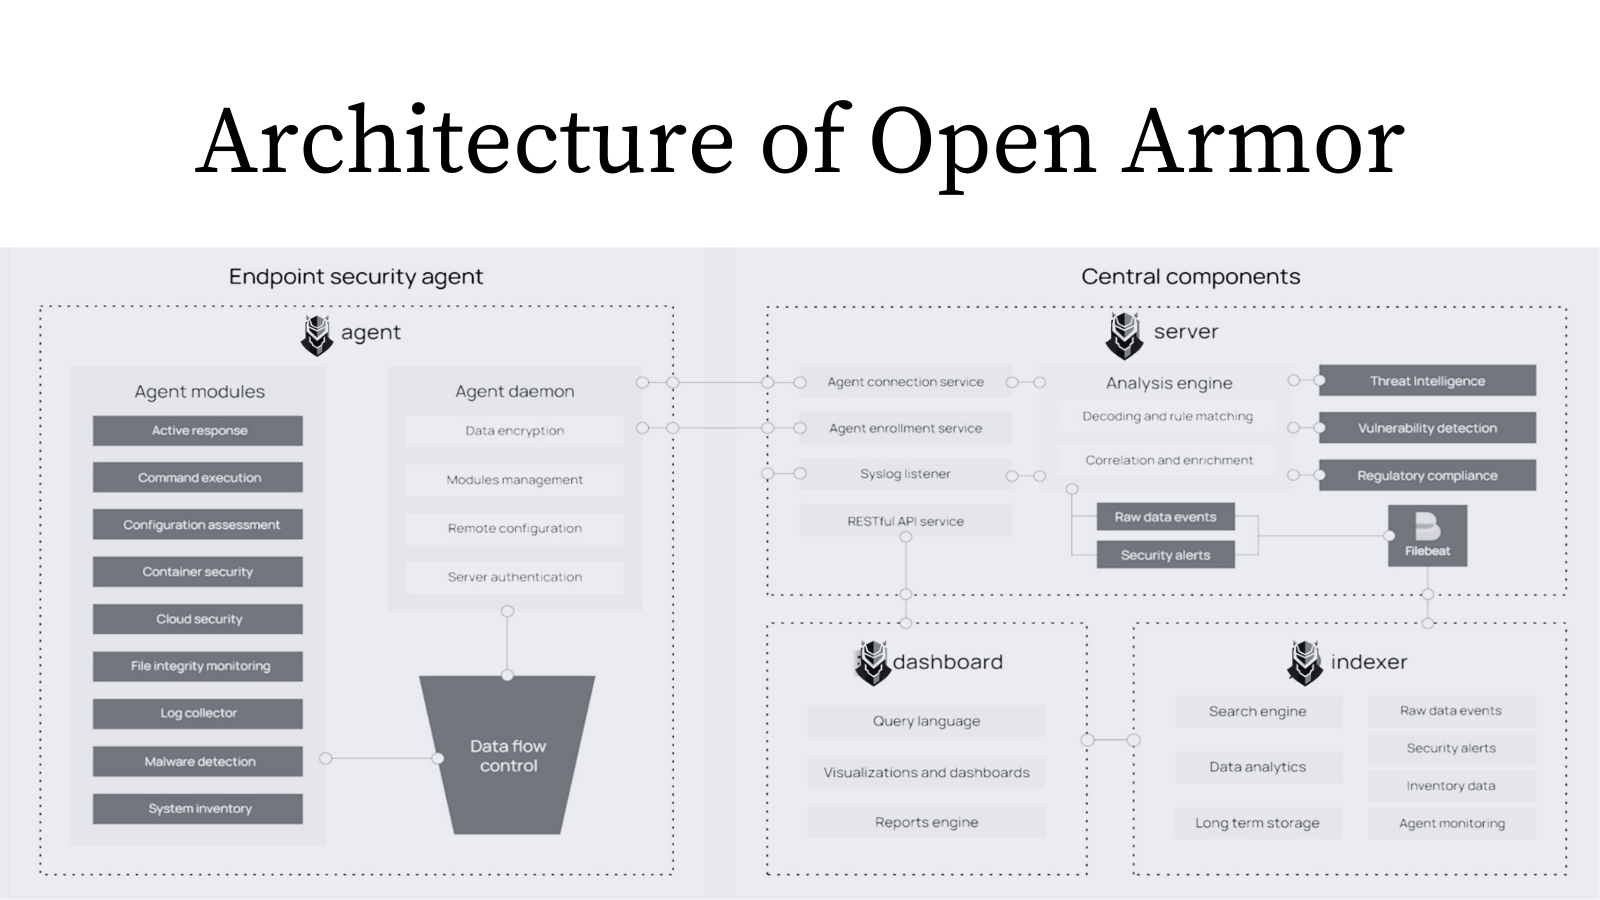
\includegraphics[width=1\linewidth]{OpenArmor_Architecture.png}
    \caption{OpenArmor High-Level Architecture}
    \label{fig:openarmor-architecture}
\end{figure}

\begin{figure}[h]
    \centering
    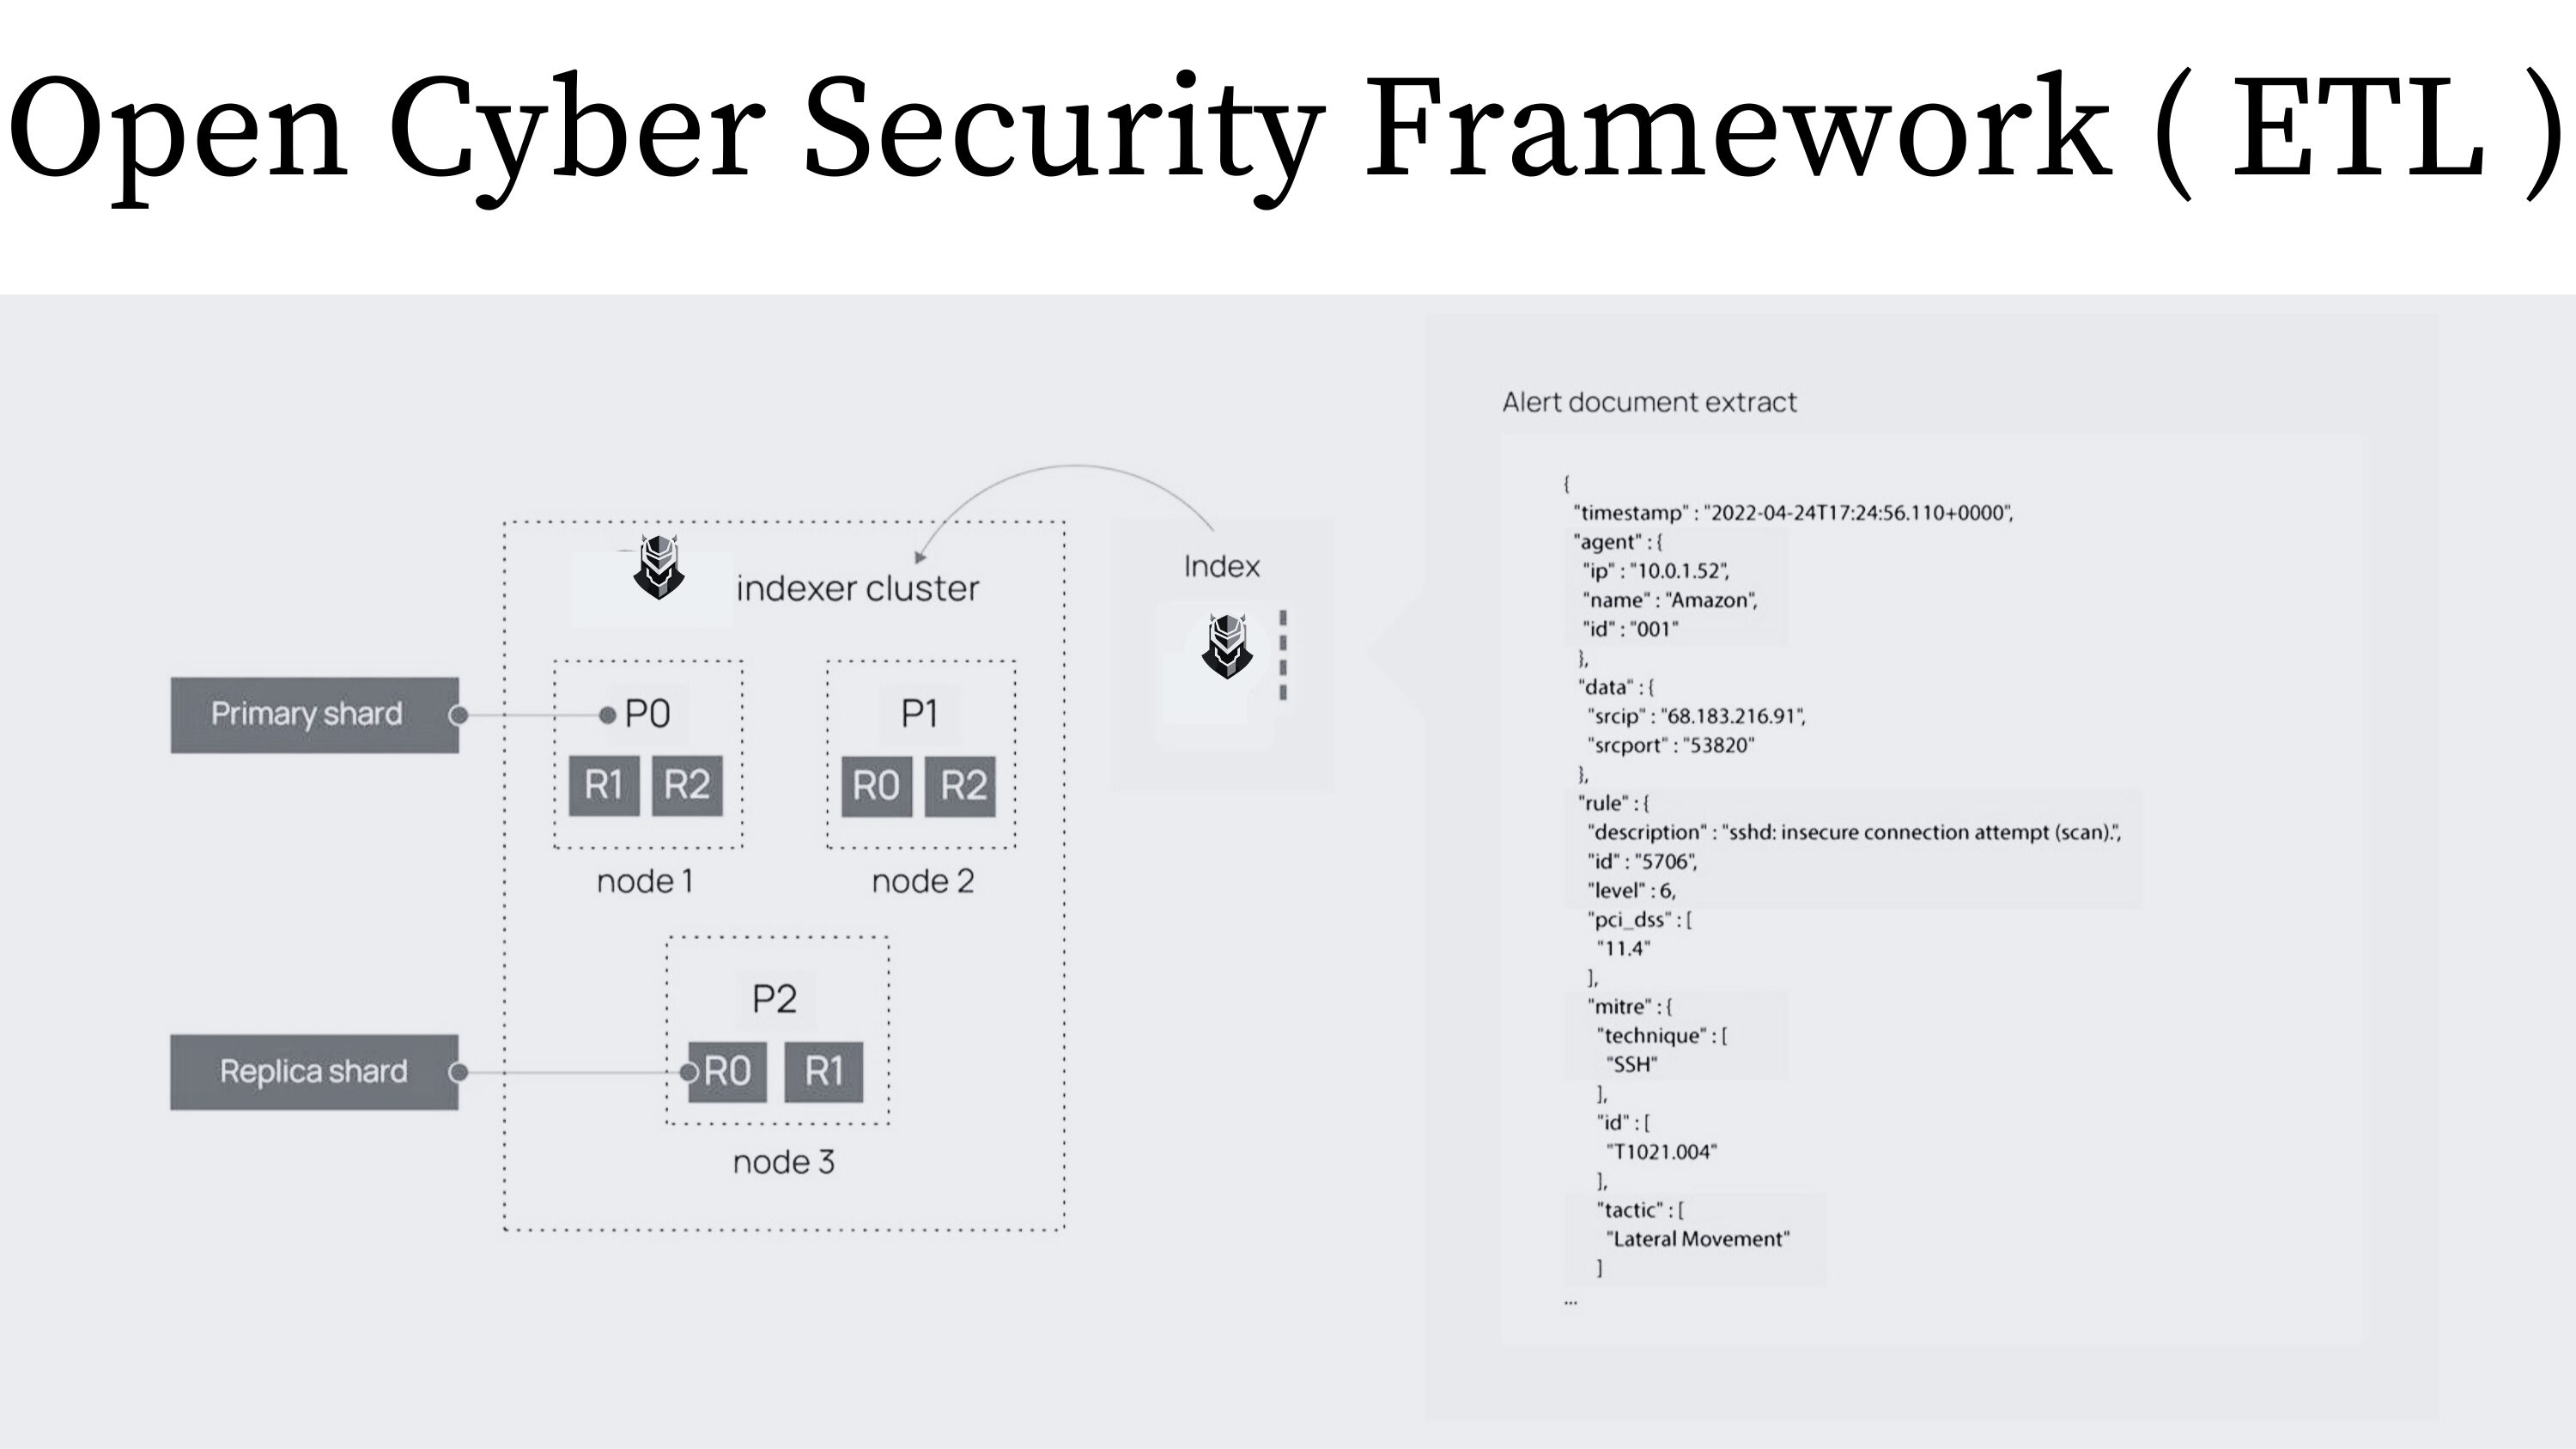
\includegraphics[width=1\linewidth]{ocsf-etl.png}
    \caption{OCSF Schema Parsing Architecture}
    \label{fig:ocsf-architecture}
\end{figure}

\begin{figure}[h]
    \centering
    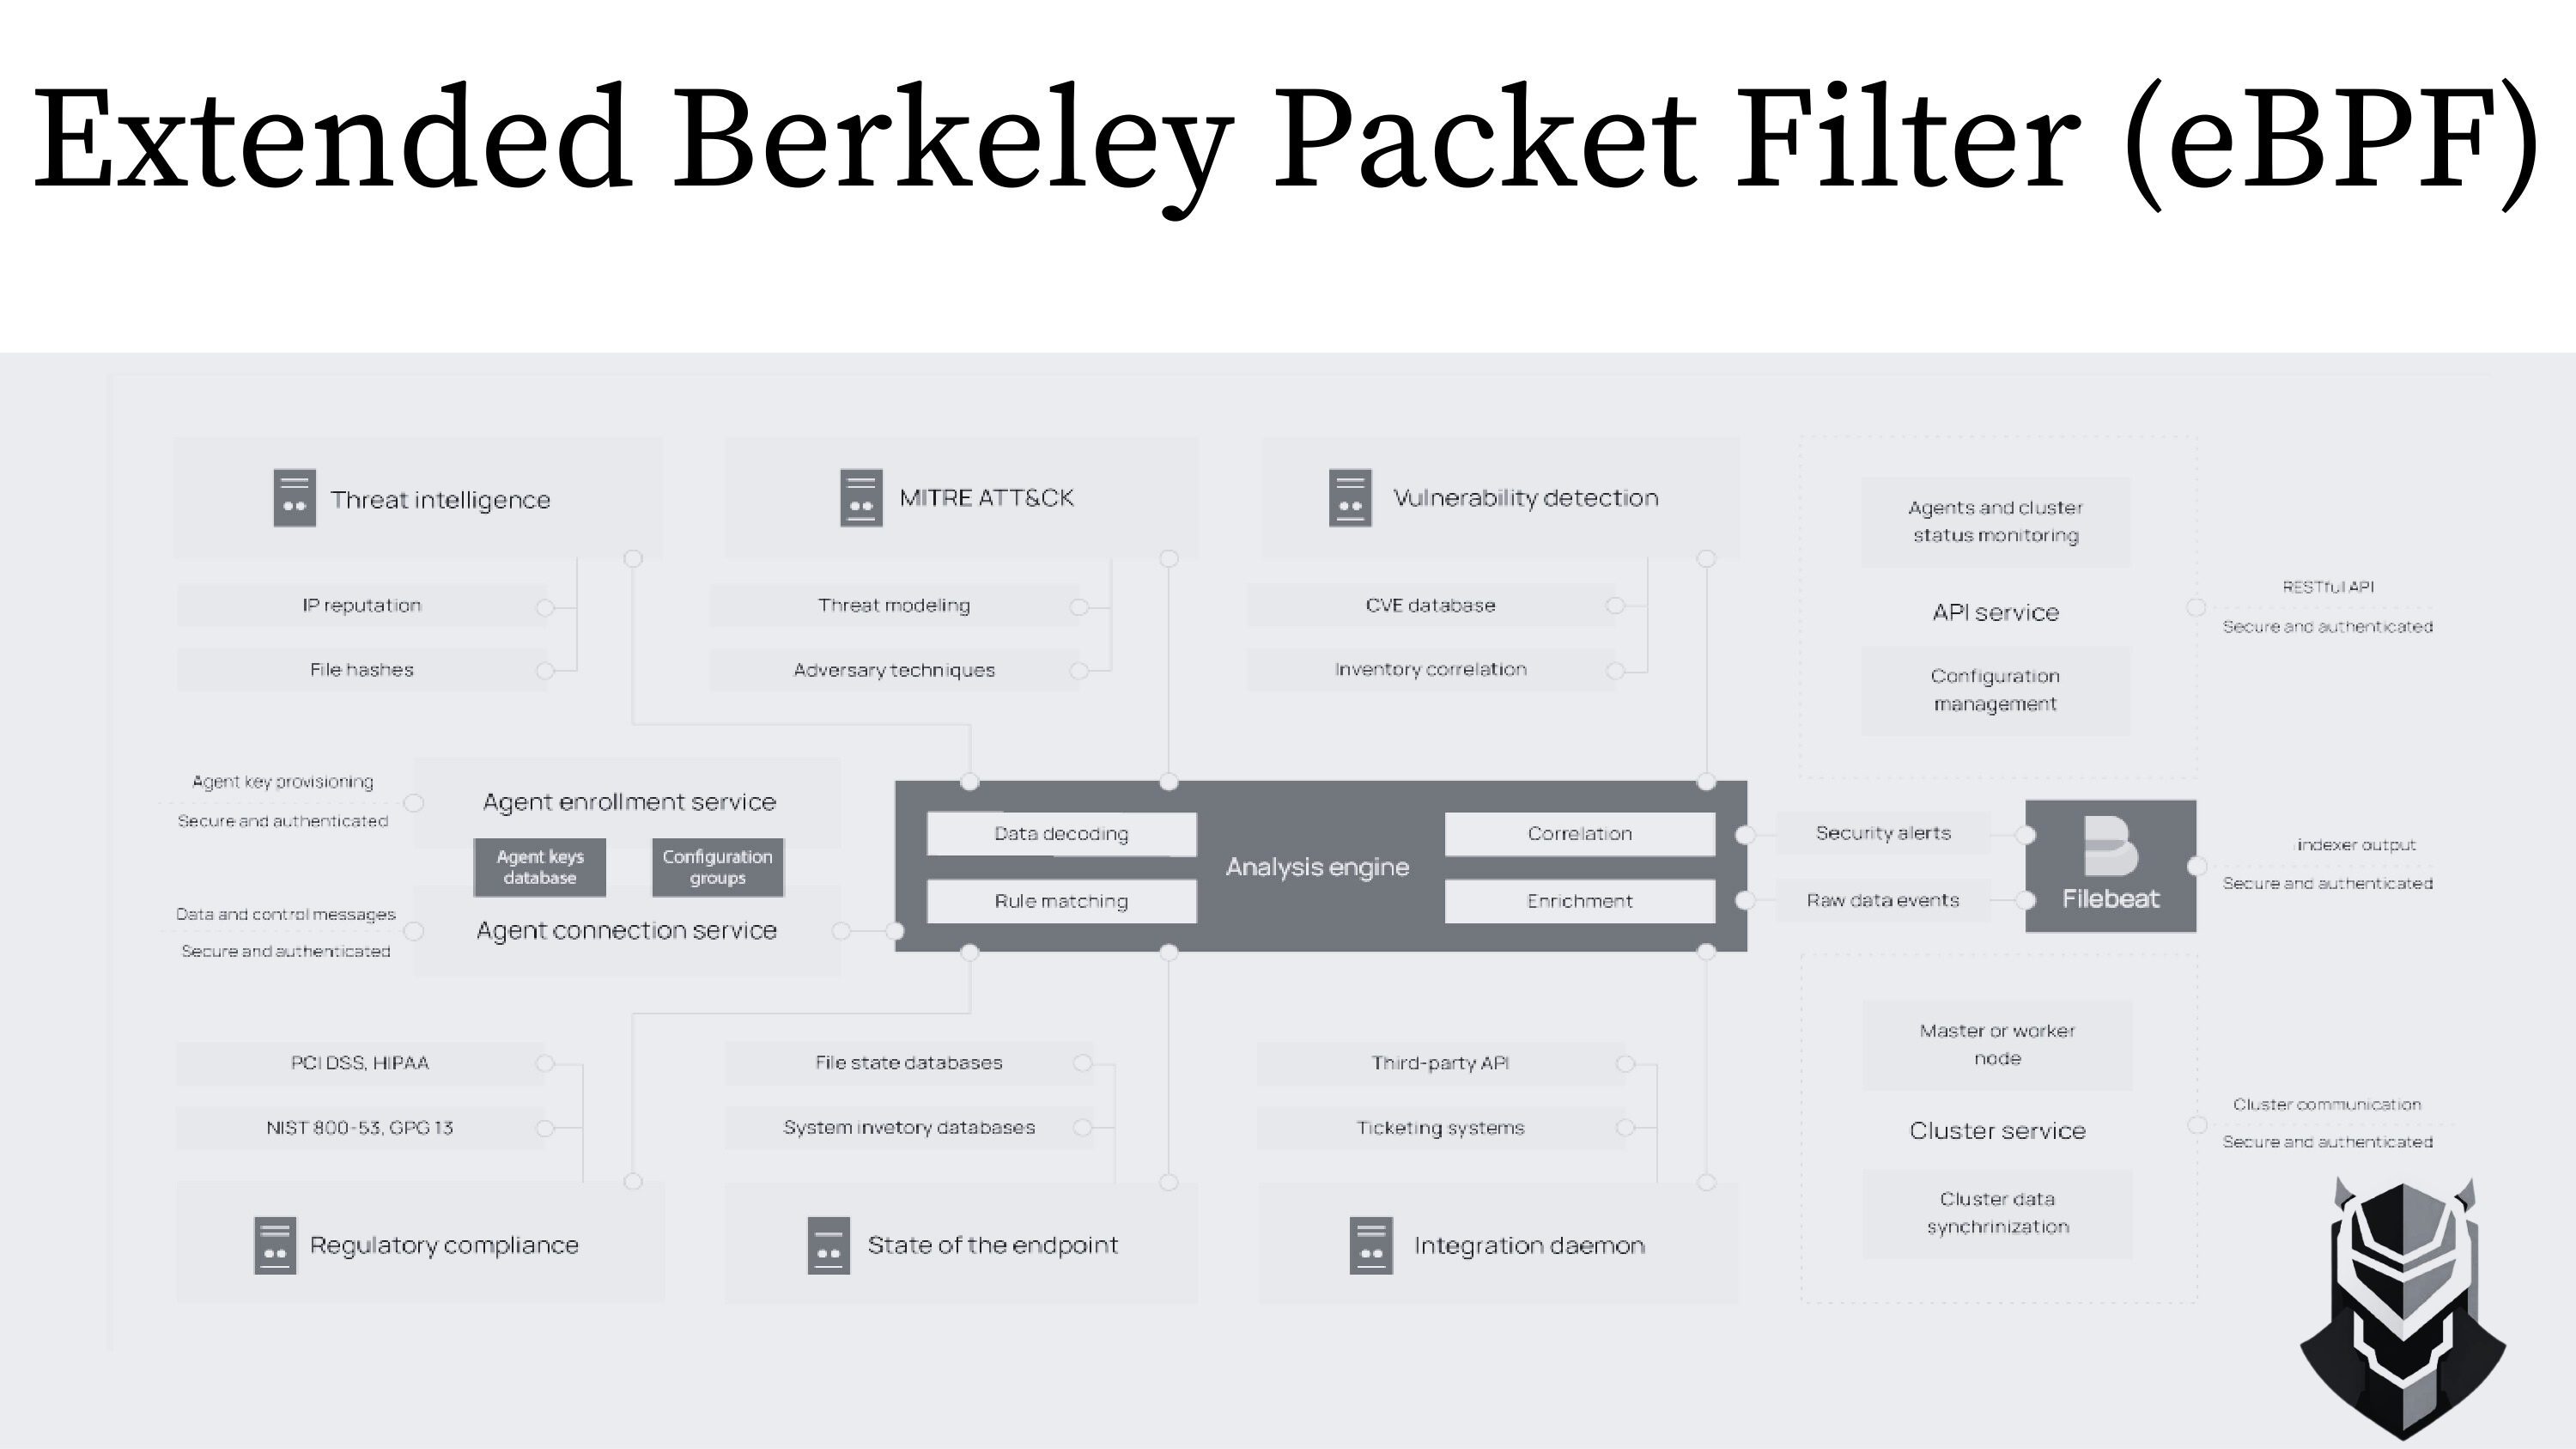
\includegraphics[width=1\linewidth]{ebpf-server.png}
    \caption{Extended Berkeley Packet Filter (eBPF) Server Side Architecture}
    \label{fig:ebpf-architecture}
\end{figure}

\begin{figure}[h]
    \centering
    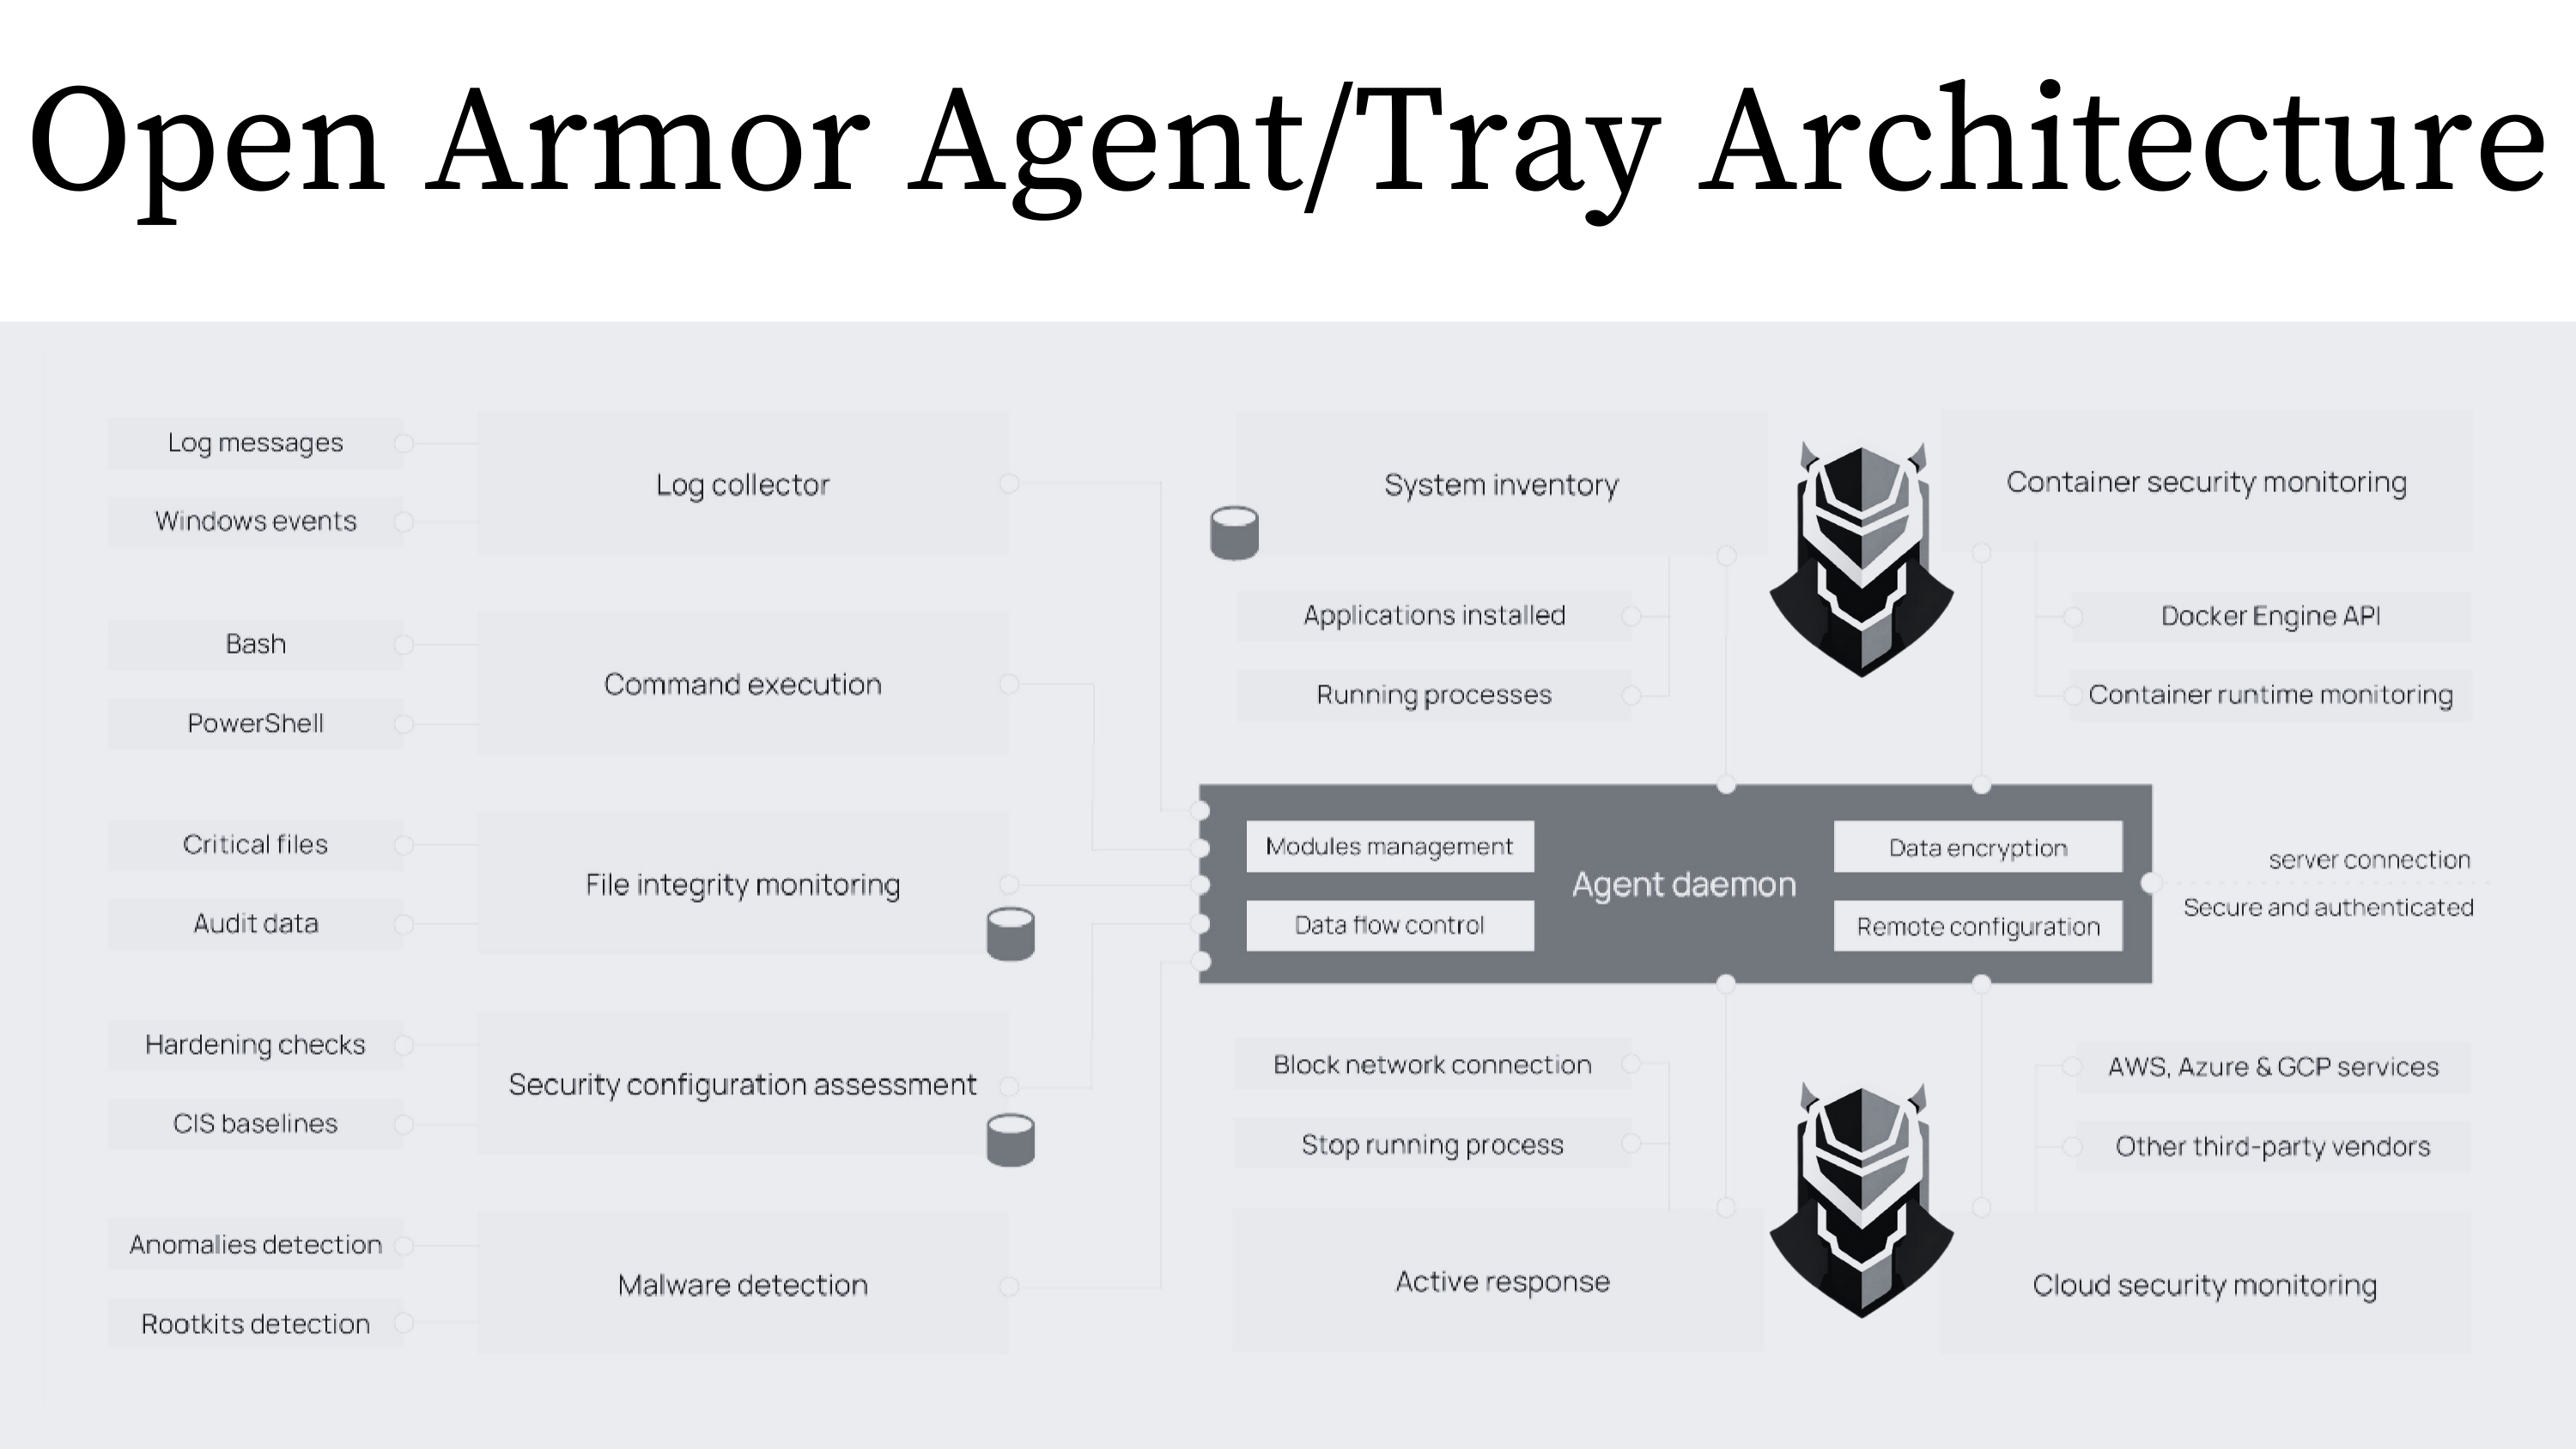
\includegraphics[width=1\linewidth]{openarmor-agent.png}
    \caption{Open Armor Agent Side Architecture}
    \label{fig:agent-architecture}
\end{figure}

\section{External Interfaces}

\subsection{User Interfaces}
OpenArmor's web-based dashboard serves as the primary user interface, incorporating:

\begin{itemize}
    \item Responsive design adhering to modern UI/UX principles
    \item Role-based access control for different user types
    \item Real-time event viewer with advanced filtering capabilities
    \item Customizable dashboards for various security metrics
    \item Interactive threat investigation tools
    \item Configuration management for agents and detection rules
\end{itemize}

\subsection{Hardware Interfaces}
OpenArmor interfaces with various hardware components, including:

\begin{itemize}
    \item Network Interface Cards (NICs) for packet capture and analysis
    \item Storage devices for log retention and database management
    \item Hardware Security Modules (HSMs) for secure key storage
    \item IPMI-enabled devices for out-of-band management in server environments
\end{itemize}

\subsection{Software Interfaces}
OpenArmor integrates with and extends several key software components:

\begin{itemize}
    \item Wazuh: Leveraging its HIDS capabilities and agent network
    \item OSquery: Utilizing its SQL-like interface for system state queries
    \item Sysmon: Incorporating its detailed Windows event logging
    \item SIEM Systems: Integration via OCSF-standardized logs
    \item Threat Intelligence Platforms: For IoC and threat data ingestion
\end{itemize}

APIs are provided for:
\begin{itemize}
    \item RESTful data access and management
    \item Webhook integrations for real-time alert notifications
    \item Custom plugin development and extension
\end{itemize}

\subsection{Communication Interfaces}
OpenArmor supports various communication protocols:

\begin{itemize}
    \item TLS-encrypted agent-server communication
    \item HTTPS for web interface access
    \item SSH for secure remote management
    \item Syslog for log ingestion from external sources
    \item MQTT for IoT device communication and monitoring
\end{itemize}

\section{System Features}

\subsection{eBPF-Enhanced Kernel Space Logging}
\subsubsection{Description and Priority}
High-priority feature for efficient, low-overhead kernel-level logging using eBPF technology.

\subsubsection{Stimulus/Response Sequences}
\begin{itemize}
    \item eBPF programs continuously monitor kernel events
    \item Relevant events are captured and streamed to the OpenArmor Core
    \item OpenArmor processes and correlates kernel-level data with other sources
\end{itemize}

\subsubsection{Functional Requirements}
\begin{itemize}
    \item REQ-1: Implement eBPF programs for comprehensive kernel event monitoring
    \item REQ-2: Develop a high-performance event streaming mechanism
    \item REQ-3: Create an extensible framework for custom eBPF programs
\end{itemize}

\subsection{OCSF Standardization and Integration}
\subsubsection{Description and Priority}
Critical feature for ensuring interoperability and standardized log formats across the system.

\subsubsection{Stimulus/Response Sequences}
\begin{itemize}
    \item Logs from various sources (Wazuh, OSquery, Sysmon, eBPF) are ingested
    \item OCSF Normalization Layer processes and standardizes the logs
    \item Standardized logs are made available for analysis and export
\end{itemize}

\subsubsection{Functional Requirements}
\begin{itemize}
    \item REQ-4: Develop adaptors for Wazuh, OSquery, and Sysmon log formats
    \item REQ-5: Implement OCSF schema mapping and validation
    \item REQ-6: Create an API for exporting OCSF-compliant logs to external systems
\end{itemize}

\subsection{AI-Driven Threat Detection}
\subsubsection{Description and Priority}
High-priority feature leveraging machine learning for advanced threat detection and analysis.

\subsubsection{Stimulus/Response Sequences}
\begin{itemize}
    \item AI Analytics Module continuously processes normalized log data
    \item Anomalies and potential threats are identified in real-time
    \item Alerts are generated and prioritized based on severity and confidence
    \item Threat intelligence is updated based on new findings
\end{itemize}

\subsubsection{Functional Requirements}
\begin{itemize}
    \item REQ-7: Develop and train ML models for anomaly detection
    \item REQ-8: Implement a real-time scoring system for threat prioritization
    \item REQ-9: Create an adaptive learning mechanism to improve detection over time
    \item REQ-10: Integrate with external threat intelligence sources for enhanced context
\end{itemize}

\subsection{Unified Query and Response System}
\subsubsection{Description and Priority}
Important feature providing a centralized interface for querying and responding to security events across all integrated components.

\subsubsection{Stimulus/Response Sequences}
\begin{itemize}
    \item User or automated system submits a query through the interface
    \item Query is distributed to relevant components (OSquery, Wazuh, eBPF engine)
    \item Results are collated, normalized, and presented to the user
    \item Automated response actions are suggested or executed based on query results
\end{itemize}

\subsubsection{Functional Requirements}
\begin{itemize}
    \item REQ-11: Develop a unified query language encompassing all data sources
    \item REQ-12: Implement query distribution and result aggregation mechanisms
    \item REQ-13: Create an automated response framework with customizable playbooks
    \item REQ-14: Provide an API for integrating the query system with external tools
\end{itemize}

\section{Data Design}
OpenArmor's data model is designed to efficiently store and process security events from various sources. Key components include:

\begin{itemize}
    \item Event Database: Stores normalized OCSF-compliant log entries
    \item Configuration Database: Manages system and agent configurations
    \item Threat Intelligence Database: Stores IoCs and threat patterns
    \item Machine Learning Model Storage: Retains trained ML models and their metadata
\end{itemize}

\section{Security and Privacy Design}
Security is paramount in OpenArmor's design, incorporating:

\begin{itemize}
    \item End-to-end encryption for all communications
    \item Secure key management using HSMs where available
    \item Role-based access control for all system functions
    \item Audit logging of all administrative actions
    \item Data anonymization techniques for privacy-sensitive information
    \item Regular security assessments and penetration testing
\end{itemize}

\section{Performance}
OpenArmor is designed to meet high-performance requirements:

\begin{itemize}
    \item Scalability to handle up to 100,000 endpoints in a single deployment
    \item Processing capability of up to 100,000 events per second
    \item Sub-second alert generation for critical threats
    \item Web interface response time under 2 seconds for most operations
    \item Efficient resource utilization on monitored systems (< 5% CPU, < 256MB RAM)
\end{itemize}

\section{Conclusion}
This system design outlines the architecture, interfaces, and key features of OpenArmor, integrating the strengths of Wazuh, OSquery, and Sysmon with innovative eBPF and AI-driven capabilities. The design emphasizes scalability, performance, and extensibility, positioning OpenArmor as a next-generation cybersecurity solution capable of addressing complex and evolving threat landscapes.
\chapter{Methodology}

The development of OpenArmor, an advanced cybersecurity solution leveraging AI and advanced logging techniques, followed a systematic approach that integrates cutting-edge technologies with established security tools. Our methodology can be divided into four main phases: data acquisition, data integration and normalization, data processing and analysis, and threat detection and response.

\section{Data Acquisition Phase}

This phase focused on gathering comprehensive system and network data from multiple sources:

\subsection{eBPF-based Kernel Monitoring}
We implemented eBPF (Extended Berkeley Packet Filter) programs for efficient kernel-level logging and monitoring of system activities. eBPF provides:
\begin{itemize}
    \item Low-overhead, real-time monitoring of system calls, network events, and file operations
    \item Safe execution of sandboxed programs in the Linux kernel
    \item Customizable data collection points for comprehensive visibility
\end{itemize}

\subsection{Integration with Existing Security Tools}
We leveraged the capabilities of established security tools:
\begin{itemize}
    \item Wazuh: For host-based intrusion detection and file integrity monitoring
    \item OSquery: To query endpoint state information using SQL-like syntax
    \item Sysmon: For detailed Windows event logging and process monitoring
\end{itemize}

\subsection{Network Traffic Analysis}
We implemented network traffic capture and analysis using:
\begin{itemize}
    \item libpcap for efficient packet capture
    \item Deep packet inspection techniques for protocol analysis
    \item NetFlow/IPFIX collection for network flow monitoring
\end{itemize}

\section{Data Integration and Normalization Phase}

In this phase, we focused on centralizing and standardizing the diverse data sources:

\subsection{OCSF Standardization}
We adopted the OCSF (Open Cybersecurity Schema Framework) to structure and normalize log data:
\begin{itemize}
    \item Developed custom parsers for eBPF, Wazuh, OSquery, and Sysmon data
    \item Implemented OCSF schema mapping and validation
    \item Created an extensible framework for adding new data source adapters
\end{itemize}

\subsection{Data Enrichment}
We enriched the normalized data with contextual information:
\begin{itemize}
    \item Geo-location data for IP addresses
    \item Threat intelligence feed integration for known IoCs
    \item Asset management integration for system context
\end{itemize}

\section{Data Processing and Analysis Phase}

This phase involved preparing the data for analysis and implementing advanced analytics:

\subsection{Data Preprocessing}
We applied various preprocessing techniques to ensure data quality:
\begin{itemize}
    \item Feature extraction and selection
    \item Handling of missing data and outliers
    \item Data normalization and scaling
\end{itemize}

\subsection{Machine Learning Pipeline}
We developed a comprehensive machine learning pipeline:
\begin{itemize}
    \item Unsupervised learning for anomaly detection:
    \begin{itemize}
        \item Isolation Forest for outlier detection
        \item DBSCAN for density-based clustering of security events
    \end{itemize}
    \item Supervised learning for threat classification:
    \begin{itemize}
        \item Random Forest for multi-class threat categorization
        \item Gradient Boosting for binary classification of malicious/benign events
    \end{itemize}
    \item Deep learning models for complex pattern recognition:
    \begin{itemize}
        \item LSTM networks for sequence-based anomaly detection in log data
        \item Autoencoders for dimensionality reduction and feature learning
    \end{itemize}
\end{itemize}

\subsection{Real-time Analytics}
We implemented streaming analytics capabilities:
\begin{itemize}
    \item Apache Kafka for high-throughput event streaming
    \item Apache Flink for real-time data processing and analytics
    \item Custom sliding window algorithms for time-series analysis
\end{itemize}

\section{Threat Detection and Response Phase}

This phase focused on identifying threats and facilitating rapid response:

\subsection{Automated Threat Detection}
We developed a multi-layered threat detection system:
\begin{itemize}
    \item Rule-based detection using Wazuh's capabilities
    \item Anomaly-based detection using our machine learning models
    \item Behavior-based detection for identifying complex attack patterns
\end{itemize}

\subsection{Alert Prioritization and Triage}
We implemented an intelligent alert management system:
\begin{itemize}
    \item Risk scoring algorithm considering threat severity and asset criticality
    \item Alert correlation to identify related security events
    \item Automated alert enrichment with contextual information
\end{itemize}

\subsection{Automated Response}
We developed capabilities for automated threat response:
\begin{itemize}
    \item Integration with firewall and EDR solutions for automated blocking
    \item Customizable playbooks for orchestrating response actions
    \item AI-assisted decision support for complex incident response
\end{itemize}

\section{Continuous Improvement}

Throughout the development process, we implemented mechanisms for continuous improvement:
\begin{itemize}
    \item Regular model retraining to adapt to evolving threats
    \item A/B testing of detection algorithms to optimize performance
    \item Feedback loops from security analysts to improve alert quality
    \item Integration of emerging threat intelligence to enhance detection capabilities
\end{itemize}

\section{Conclusion}

The methodology employed in developing OpenArmor combines advanced technologies like eBPF and AI with the strengths of established security tools such as Wazuh, OSquery, and Sysmon. By following this comprehensive approach, we've created a robust, adaptable, and intelligent cybersecurity solution capable of providing enterprise-grade protection through continuous monitoring, automated analysis, and timely response to emerging threats.
\chapter{Implementation}

The implementation of OpenArmor follows a phased approach, integrating advanced logging techniques, AI-driven analysis, and established security tools. Each phase builds upon the previous, creating a comprehensive and intelligent cybersecurity solution.

\section{Phase 1: Advanced Logging and Data Collection}

\subsection{eBPF Logging Implementation}
\begin{itemize}
    \item Develop custom eBPF programs for efficient kernel-level event capture
    \item Implement a user-space daemon to collect and buffer eBPF events
    \item Optimize eBPF programs for minimal system overhead
    \item Create interfaces for dynamically loading and unloading eBPF programs
\end{itemize}

\subsection{Integration of Existing Security Tools}
\begin{itemize}
    \item Deploy and configure Wazuh agents for host-based intrusion detection
    \item Implement OSquery for on-demand and scheduled system state queries
    \item Set up Sysmon for detailed Windows event logging
    \item Develop adapters for each tool to feed data into OpenArmor's central system
\end{itemize}

\subsection{Network Traffic Analysis}
\begin{itemize}
    \item Implement packet capture using libpcap or similar libraries
    \item Develop modules for protocol analysis and flow record generation
    \item Set up NetFlow/IPFIX collectors for network flow monitoring
\end{itemize}

\section{Phase 2: Log Standardization and Integration}

\subsection{OCSF Standardization Implementation}
\begin{itemize}
    \item Develop parsers for eBPF, Wazuh, OSquery, and Sysmon data formats
    \item Implement OCSF schema mapping and validation logic
    \item Create a flexible framework for adding new data source adapters
    \item Set up a centralized log storage system (e.g., Elasticsearch)
\end{itemize}

\subsection{Data Enrichment Pipeline}
\begin{itemize}
    \item Integrate geolocation databases for IP address enrichment
    \item Implement connectors for threat intelligence feeds
    \item Develop an asset management integration for system context
    \item Create a modular enrichment pipeline for easy extension
\end{itemize}

\section{Phase 3: AI Log Processing}

\subsection{Data Preprocessing}
\begin{itemize}
    \item Implement feature extraction and selection algorithms
    \item Develop modules for handling missing data and outliers
    \item Create data normalization and scaling pipelines
\end{itemize}

\subsection{Machine Learning Model Development}
\begin{itemize}
    \item Implement unsupervised learning models:
    \begin{itemize}
        \item Isolation Forest for outlier detection
        \item DBSCAN for density-based clustering
    \end{itemize}
    \item Develop supervised learning models:
    \begin{itemize}
        \item Random Forest for multi-class threat categorization
        \item Gradient Boosting for binary classification
    \end{itemize}
    \item Implement deep learning models:
    \begin{itemize}
        \item LSTM networks for sequence-based anomaly detection
        \item Autoencoders for dimensionality reduction
    \end{itemize}
\end{itemize}

\subsection{Natural Language Processing}
\begin{itemize}
    \item Implement text preprocessing for log messages
    \item Develop word embedding models for log semantics
    \item Create named entity recognition for identifying key elements in logs
\end{itemize}

\section{Phase 4: Automated Threat Detection}

\subsection{Rule-Based Detection Engine}
\begin{itemize}
    \item Implement a flexible rule engine supporting complex conditions
    \item Develop an interface for easy rule creation and management
    \item Integrate Wazuh's existing rule set into OpenArmor's engine
\end{itemize}

\subsection{Anomaly Detection System}
\begin{itemize}
    \item Implement statistical anomaly detection models
    \item Develop baseline profiling for normal system behavior
    \item Create adaptive thresholding for dynamic environments
\end{itemize}

\subsection{Behavior Analytics}
\begin{itemize}
    \item Implement user and entity behavior analytics (UEBA) models
    \item Develop graph-based analysis for entity relationship mapping
    \item Create behavior-based detection for advanced persistent threats
\end{itemize}

\subsection{Threat Intelligence Integration}
\begin{itemize}
    \item Implement connectors for major threat intelligence platforms
    \item Develop a local cache for efficient IoC lookups
    \item Create a feedback mechanism to contribute to threat intelligence
\end{itemize}

\section{Phase 5: Monitoring and Response}

\subsection{Real-Time Analytics Implementation}
\begin{itemize}
    \item Set up Apache Kafka for high-throughput event streaming
    \item Implement Apache Flink jobs for real-time data processing
    \item Develop custom sliding window algorithms for time-series analysis
\end{itemize}

\subsection{Alert Management System}
\begin{itemize}
    \item Implement a risk scoring algorithm for alert prioritization
    \item Develop an alert correlation engine to identify related events
    \item Create an automated alert enrichment pipeline
\end{itemize}

\subsection{Response Automation}
\begin{itemize}
    \item Develop integrations with firewalls and EDR solutions for automated blocking
    \item Implement a playbook engine for orchestrating response actions
    \item Create an AI-assisted decision support system for complex incidents
\end{itemize}

\subsection{User Interface and Dashboards}
\begin{itemize}
    \item Develop a web-based user interface using modern frontend frameworks
    \item Implement real-time data visualization components
    \item Create role-based access control for different user types
    \item Develop customizable dashboards for various security metrics
\end{itemize}

\begin{figure}[h]
    \centering
    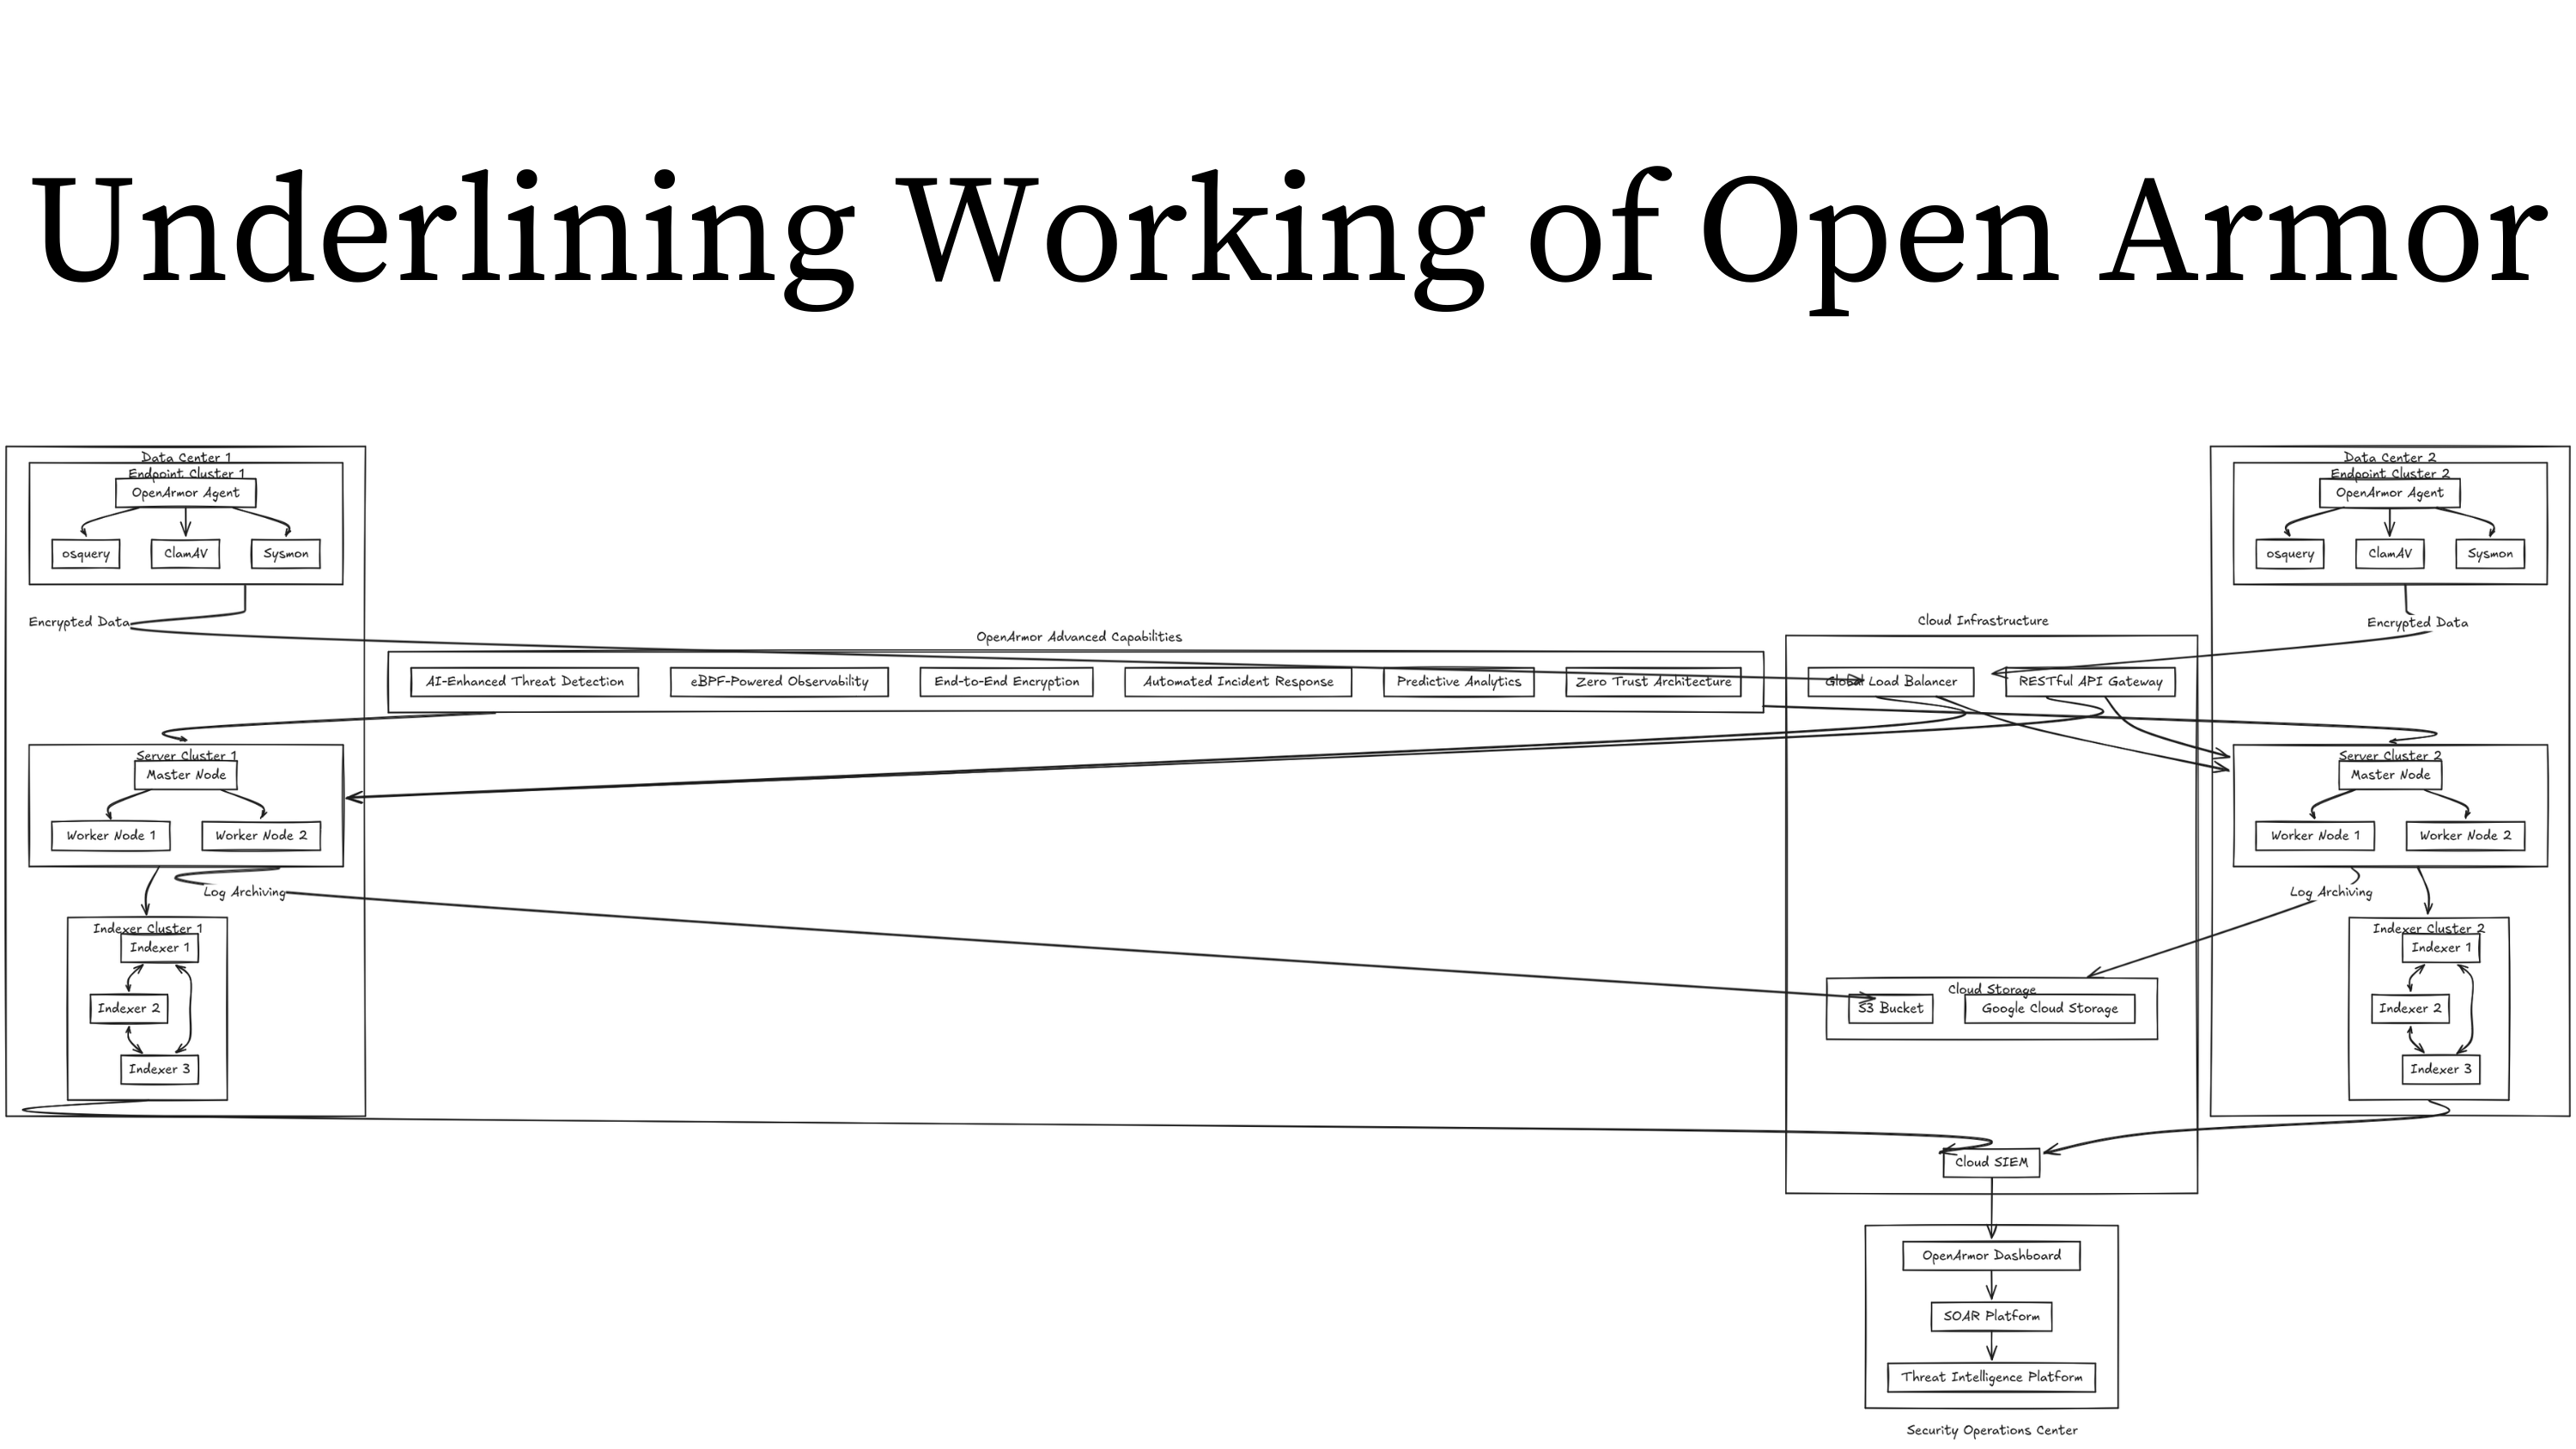
\includegraphics[width=1\linewidth]{working.png}
    \caption{OpenArmor Dashboard}
    \label{fig:openarmor-dashboard}
\end{figure}

\section{Phase 6: Continuous Improvement}

\subsection{Feedback Loop Implementation}
\begin{itemize}
    \item Develop interfaces for analysts to provide feedback on alerts
    \item Implement automated tracking of false positives and false negatives
    \item Create a system for continuous model performance evaluation
\end{itemize}

\subsection{Model Update Pipeline}
\begin{itemize}
    \item Implement automated model retraining schedules
    \item Develop A/B testing framework for new detection algorithms
    \item Create a versioning system for models and detection rules
\end{itemize}

\subsection{Threat Intelligence Gathering}
\begin{itemize}
    \item Implement a system for identifying and extracting new threat patterns
    \item Develop automated reporting of emerging threats
    \item Create a knowledge base for storing and retrieving threat information
\end{itemize}

\begin{figure}[h]
    \centering
    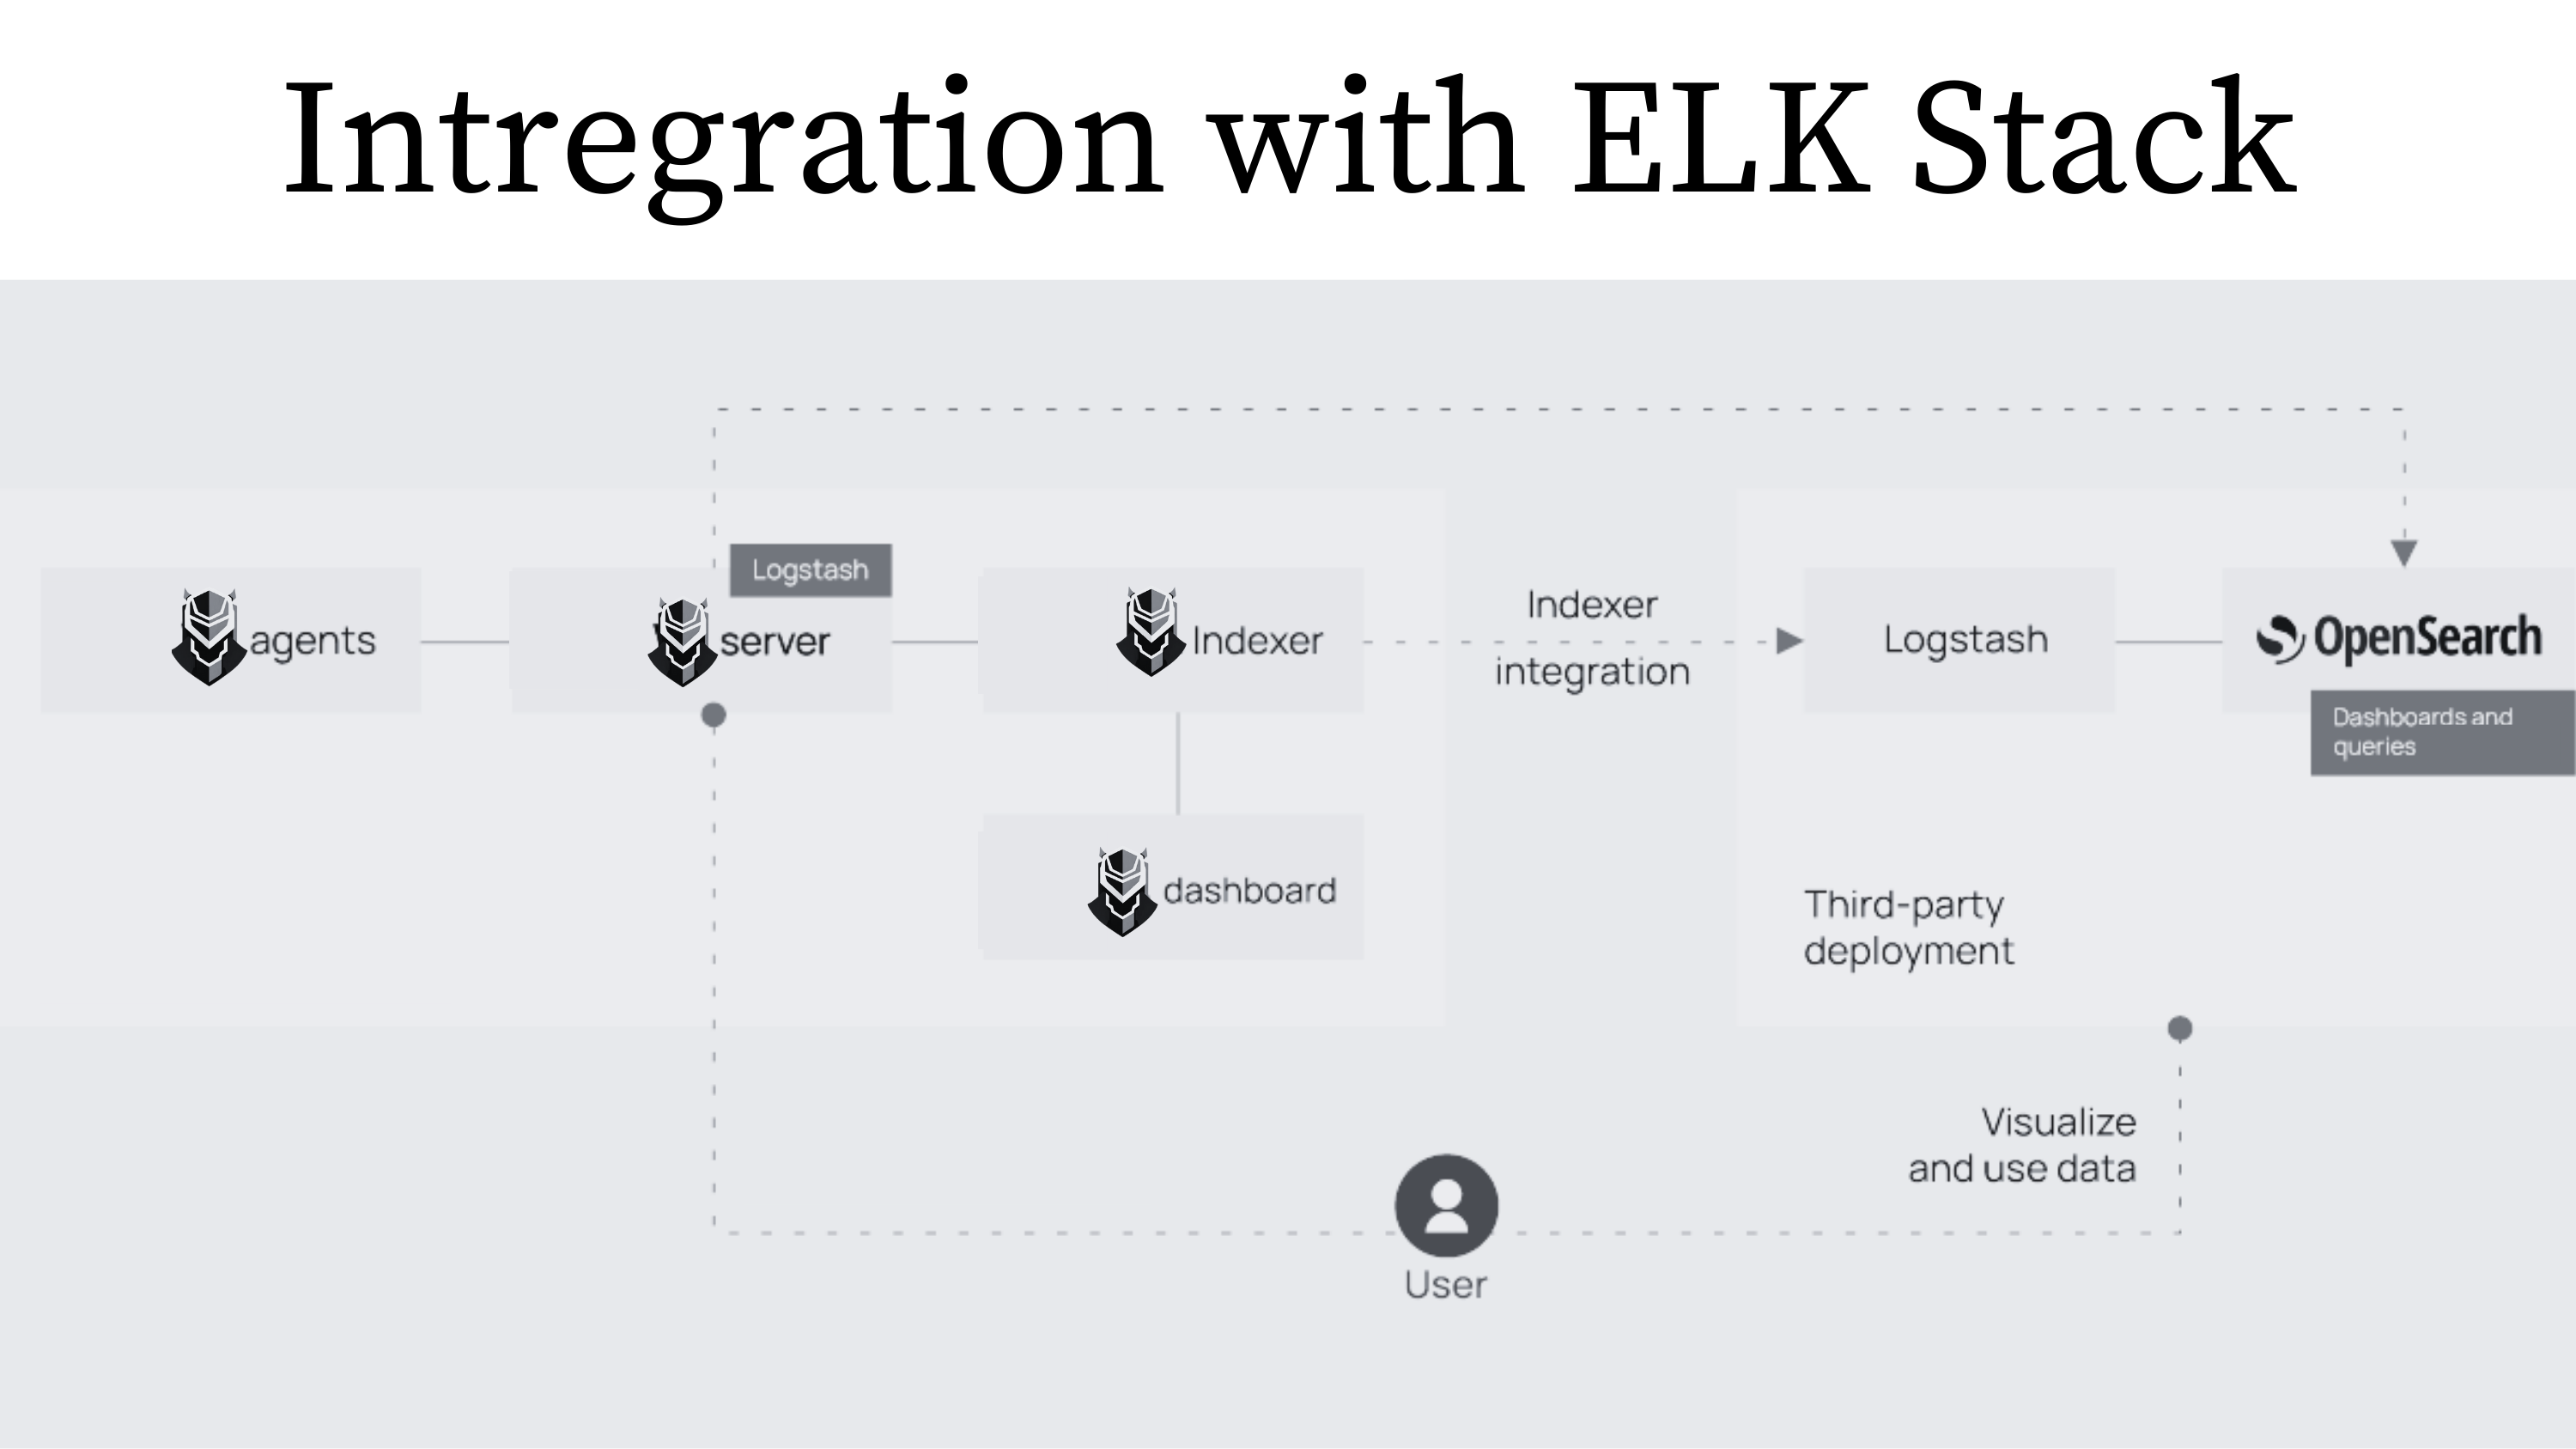
\includegraphics[width=1\linewidth]{integration-diagram-opensearch.png}
    \caption{OpenArmor Continuous Improvement Cycle for Amazon Opensearch and OpenSearch Dashboards}
    \label{fig:continuous-improvement-cycle}
\end{figure}

\section{Conclusion}

The phased implementation approach of OpenArmor ensures a systematic development of a comprehensive cybersecurity solution. By integrating advanced logging techniques, established security tools, and cutting-edge AI capabilities, OpenArmor provides a robust platform for threat detection, analysis, and response. The continuous improvement phase ensures that the system remains effective against evolving cyber threats, making OpenArmor a dynamic and adaptive security solution.
\chapter{OpenArmor Agent-Server Testing}

\section{Introduction}
This chapter outlines the testing procedures for the OpenArmor agent-server communication. It provides a structured approach to verify the functionality, security, and performance of the interaction between OpenArmor agents and the central server infrastructure.

\begin{figure}[h]
    \centering
    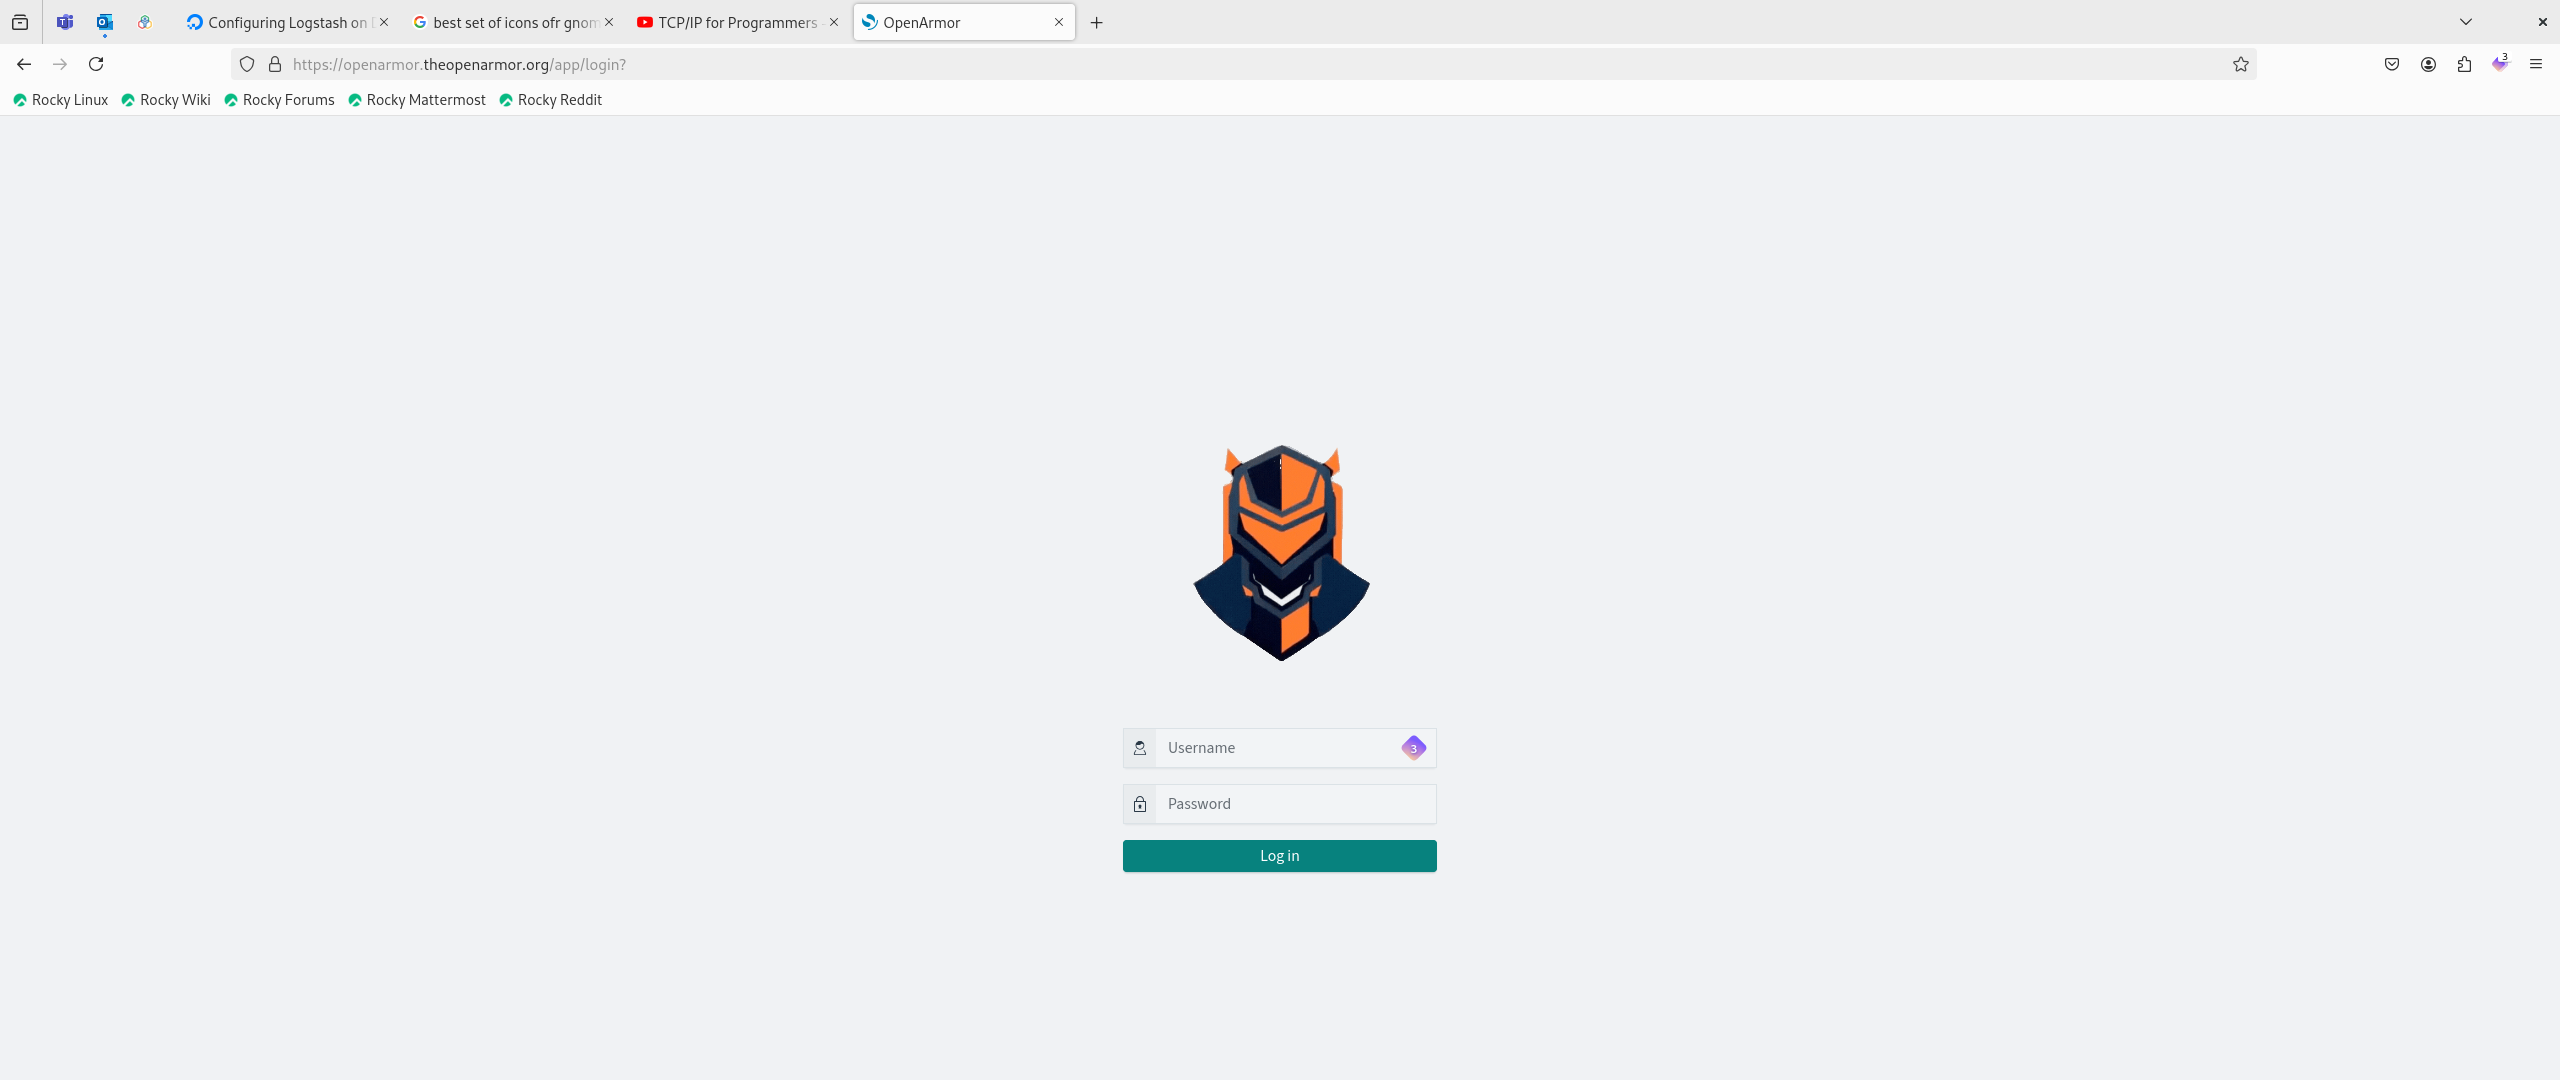
\includegraphics[width=0.8\textwidth]{openarmor-agent/1.png}
    \caption{OpenArmor Agent-Server Overview}
    \label{fig:agent-server-overview}
\end{figure}

\section{Test Environment Setup}
\subsection{Agent Setup}
\begin{enumerate}
    \item Install OpenArmor agent on test endpoints (Windows, Linux, macOS).
    \item Configure agent with test server details.
    \item Ensure all dependencies (osquery, ClamAV, Sysmon) are installed and configured.
\end{enumerate}

\begin{figure}[h]
    \centering
    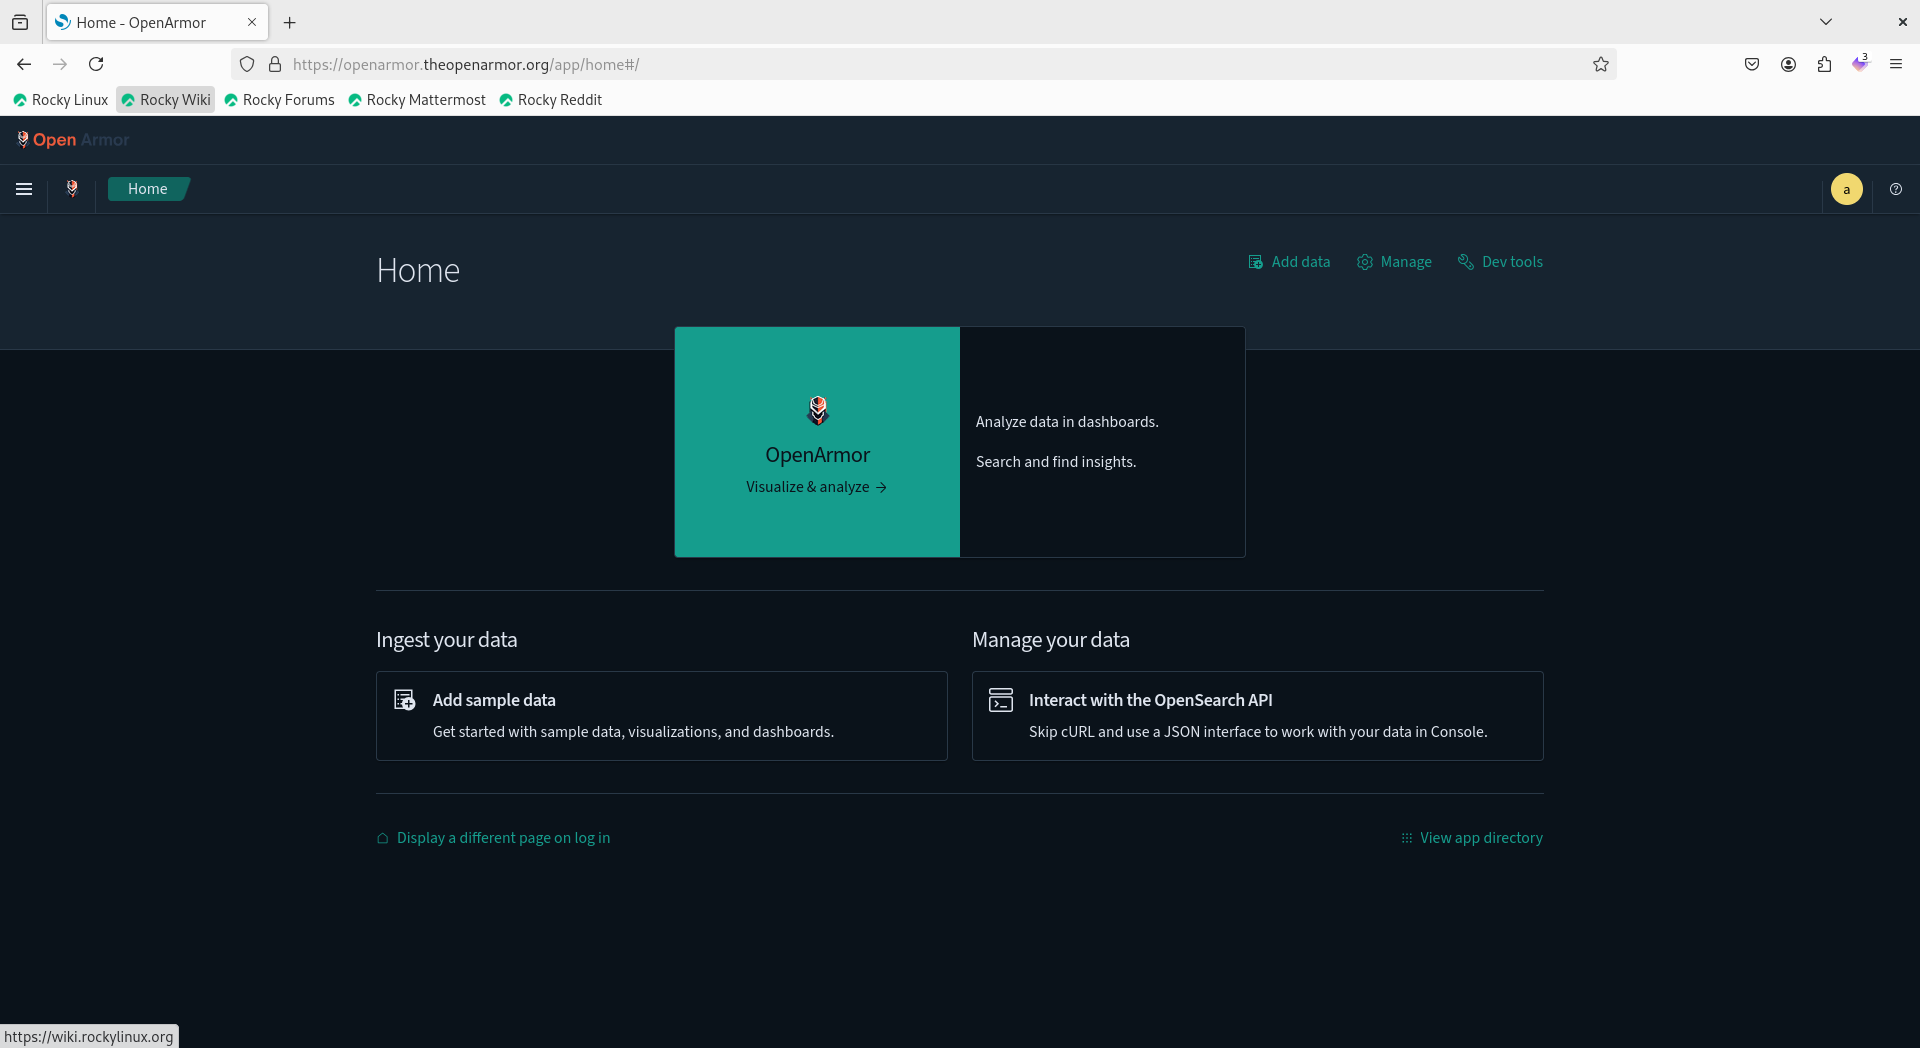
\includegraphics[width=0.7\textwidth]{openarmor-agent/2.png}
    \caption{Agent Setup Process}
    \label{fig:agent-setup}
\end{figure}

\subsection{Server Setup}
\begin{enumerate}
    \item Deploy OpenArmor server in a test environment.
    \item Configure server with test certificates and encryption keys.
    \item Set up test databases and indexers.
\end{enumerate}

\begin{figure}[h]
    \centering
    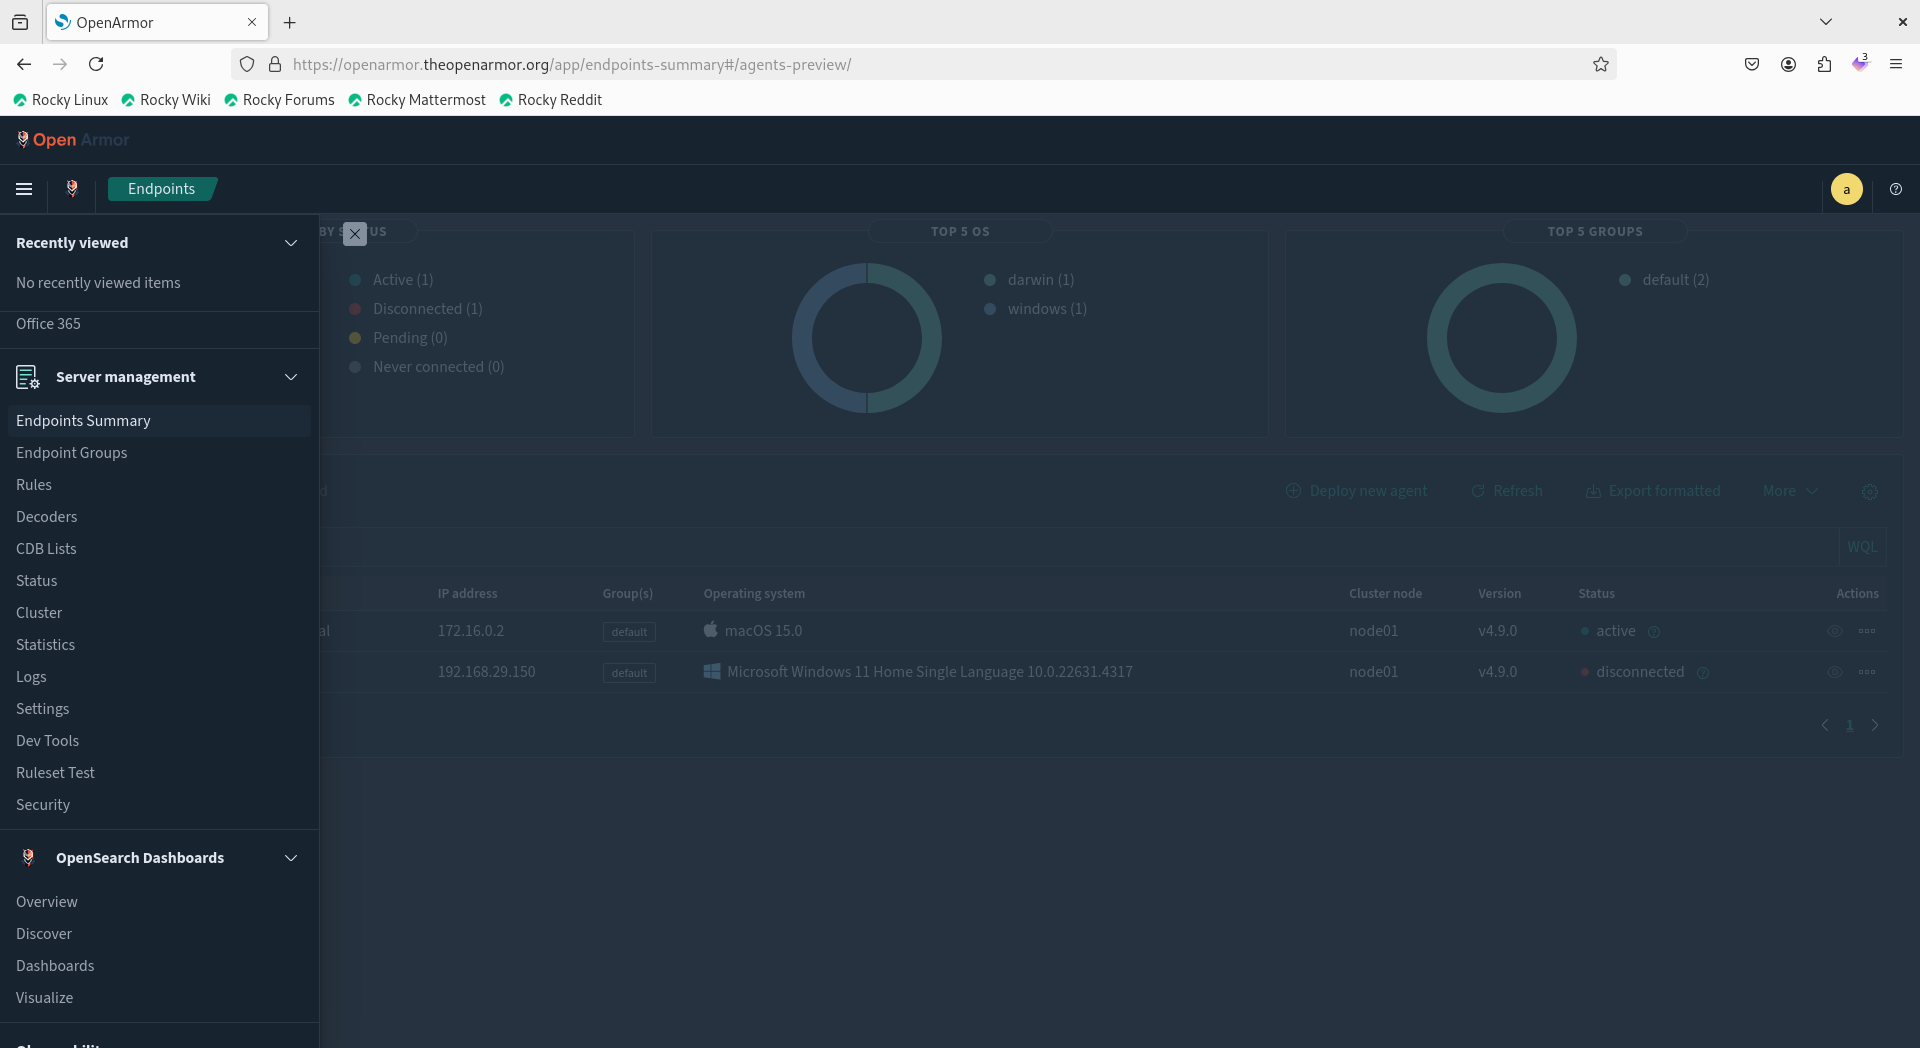
\includegraphics[width=0.7\textwidth]{openarmor-agent/3.png}
    \caption{Server Setup Configuration}
    \label{fig:server-setup}
\end{figure}

\subsection{Network Configuration}
\begin{enumerate}
    \item Configure firewalls to allow agent-server communication.
    \item Set up a test load balancer (if applicable).
    \item Prepare network monitoring tools for traffic analysis.
\end{enumerate}

\section{Functionality Testing}
\subsection{Agent Registration}
\begin{enumerate}
    \item Test new agent registration process.
    \item Verify agent appears in server's managed devices list.
    \item Check for proper agent ID assignment.
\end{enumerate}

\begin{figure}[h]
    \centering
    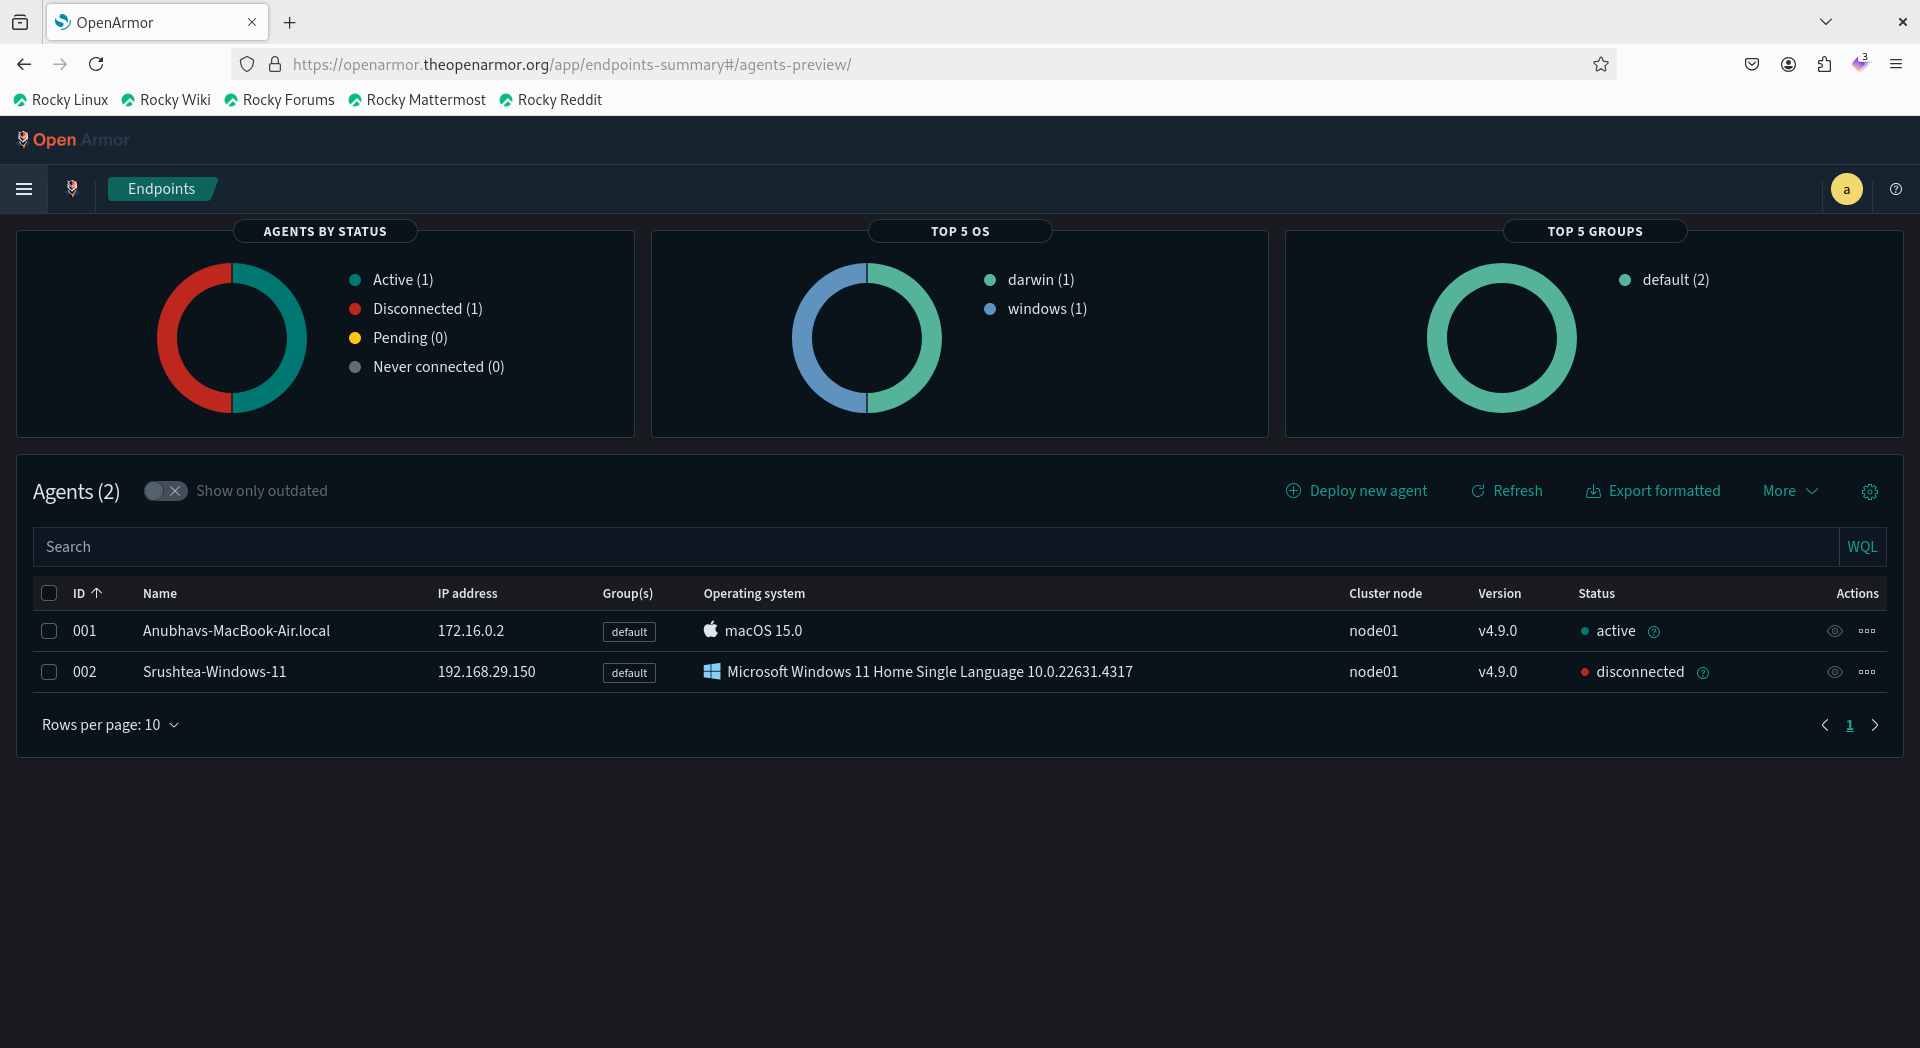
\includegraphics[width=0.8\textwidth]{openarmor-agent/4.png}
    \caption{Agent Registration Process}
    \label{fig:agent-registration}
\end{figure}

\subsection{Data Collection and Transmission}
\begin{enumerate}
    \item Trigger various events on the agent (file creation, network connection, etc.).
    \item Verify events are collected by the agent.
    \item Confirm events are successfully transmitted to the server.
    \item Check server logs for received data.
\end{enumerate}

\begin{figure}[h]
    \centering
    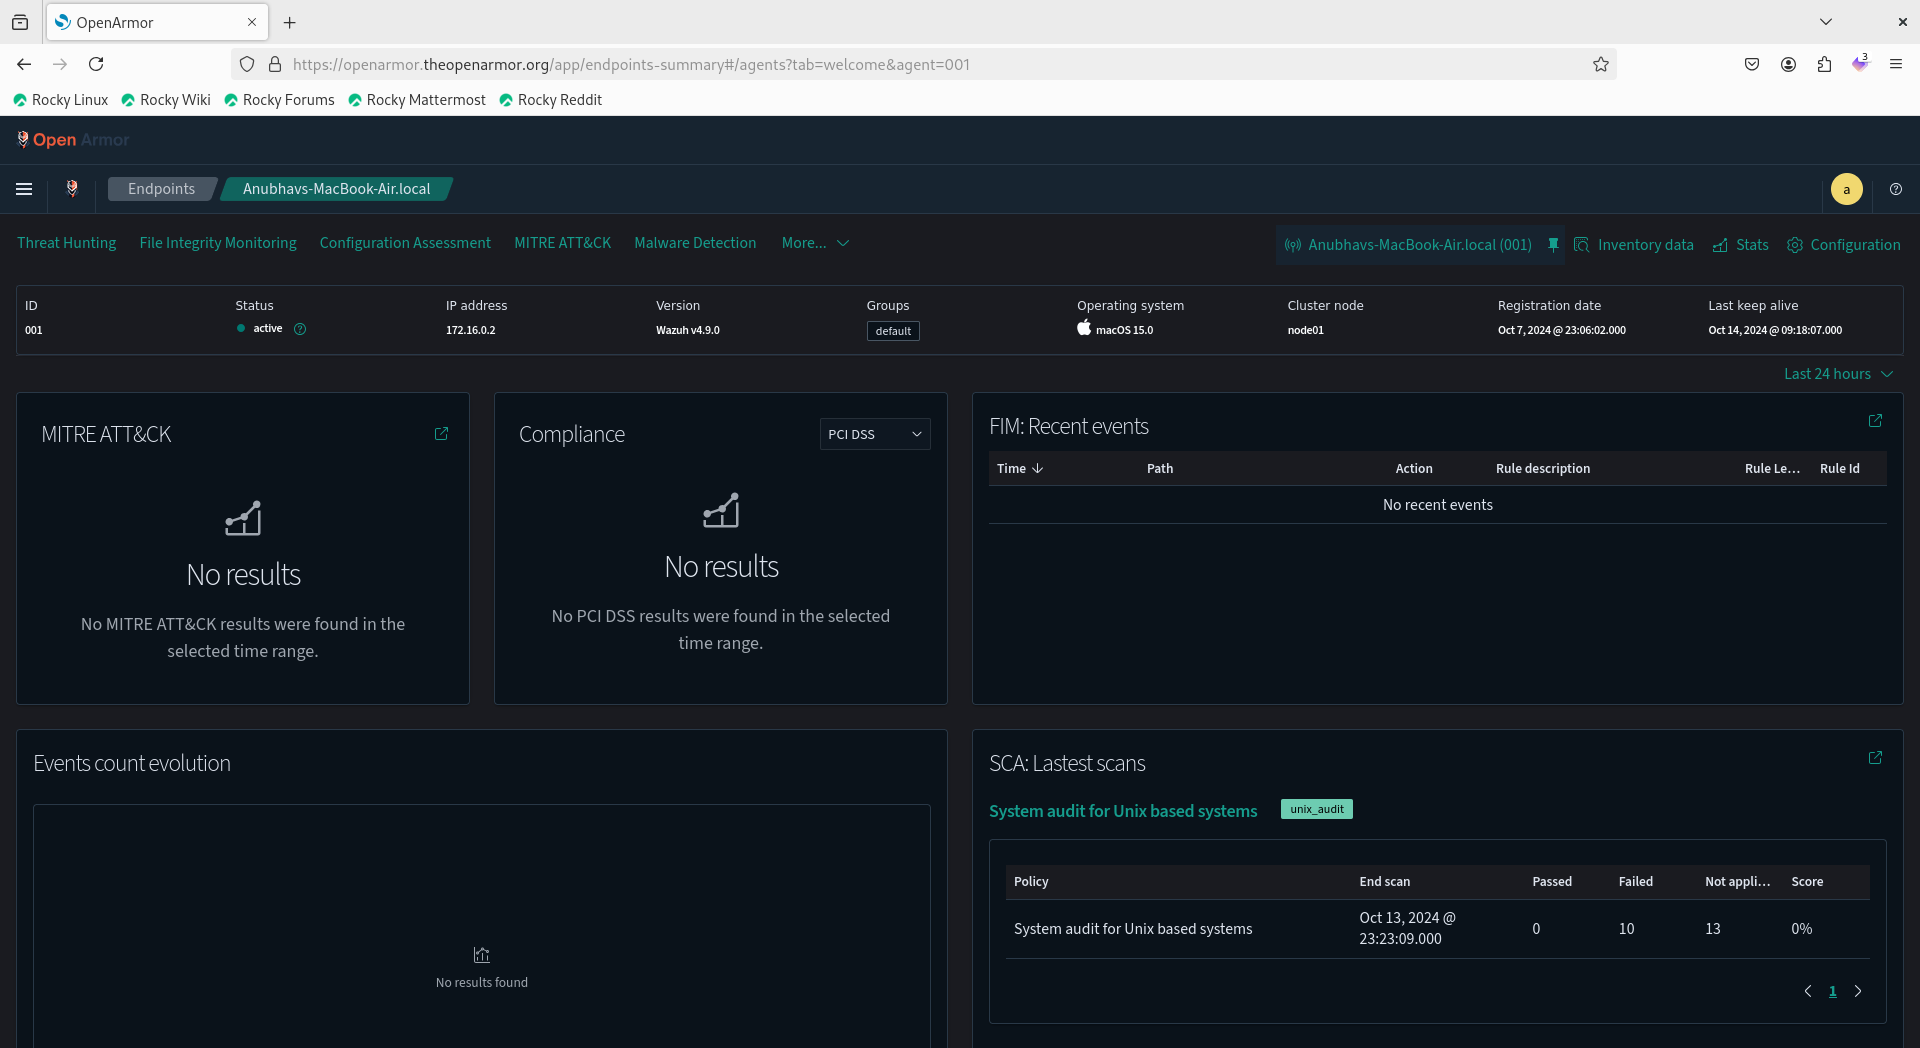
\includegraphics[width=0.7\textwidth]{openarmor-agent/5.png}
    \caption{Data Collection and Transmission Flow}
    \label{fig:data-collection}
\end{figure}

\subsection{Command and Control}
\begin{enumerate}
    \item Send configuration updates from server to agent.
    \item Issue commands (e.g., run query, update signatures) from server to agent.
    \item Verify agent acknowledges and executes commands.
    \item Check for command results reported back to the server.
\end{enumerate}

\section{Security Testing}
\subsection{Encryption}
\begin{enumerate}
    \item Capture network traffic between agent and server.
    \item Verify all traffic is encrypted (TLS inspection).
    \item Attempt to decrypt captured traffic with incorrect keys.
\end{enumerate}

\begin{figure}[h]
    \centering
    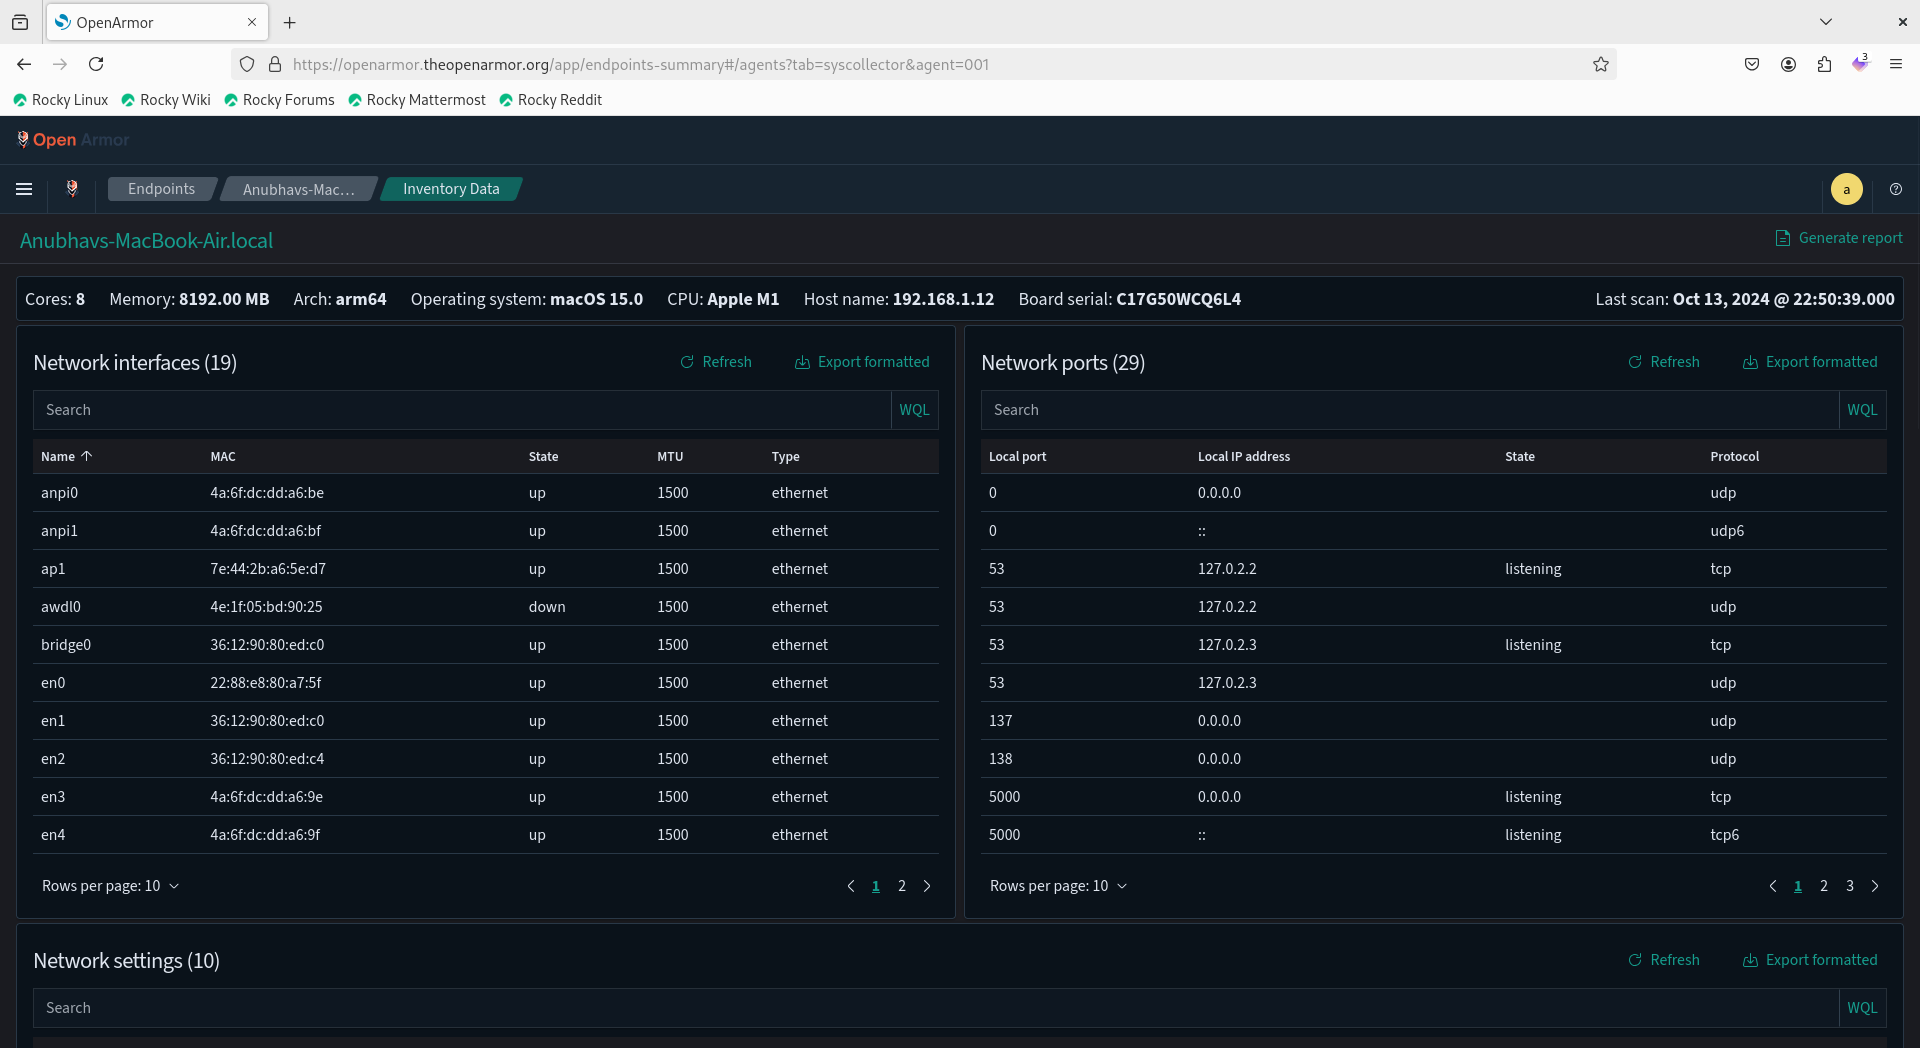
\includegraphics[width=0.8\textwidth]{openarmor-agent/6.png}
    \caption{Encryption Testing Procedure}
    \label{fig:encryption-testing}
\end{figure}

\subsection{Authentication}
\begin{enumerate}
    \item Attempt connection with invalid agent credentials.
    \item Test certificate-based authentication.
    \item Verify token-based session management.
\end{enumerate}

\subsection{Authorization}
\begin{enumerate}
    \item Test agent access to server resources with different permission levels.
    \item Attempt unauthorized command execution from agent to server.
    \item Verify data access controls on the server side.
\end{enumerate}

\section{Performance Testing}
\subsection{Load Testing}
\begin{enumerate}
    \item Simulate high event generation rate on agents.
    \item Monitor server performance under increased load.
    \item Test with multiple concurrent agent connections.
\end{enumerate}

\begin{figure}[h]
    \centering
    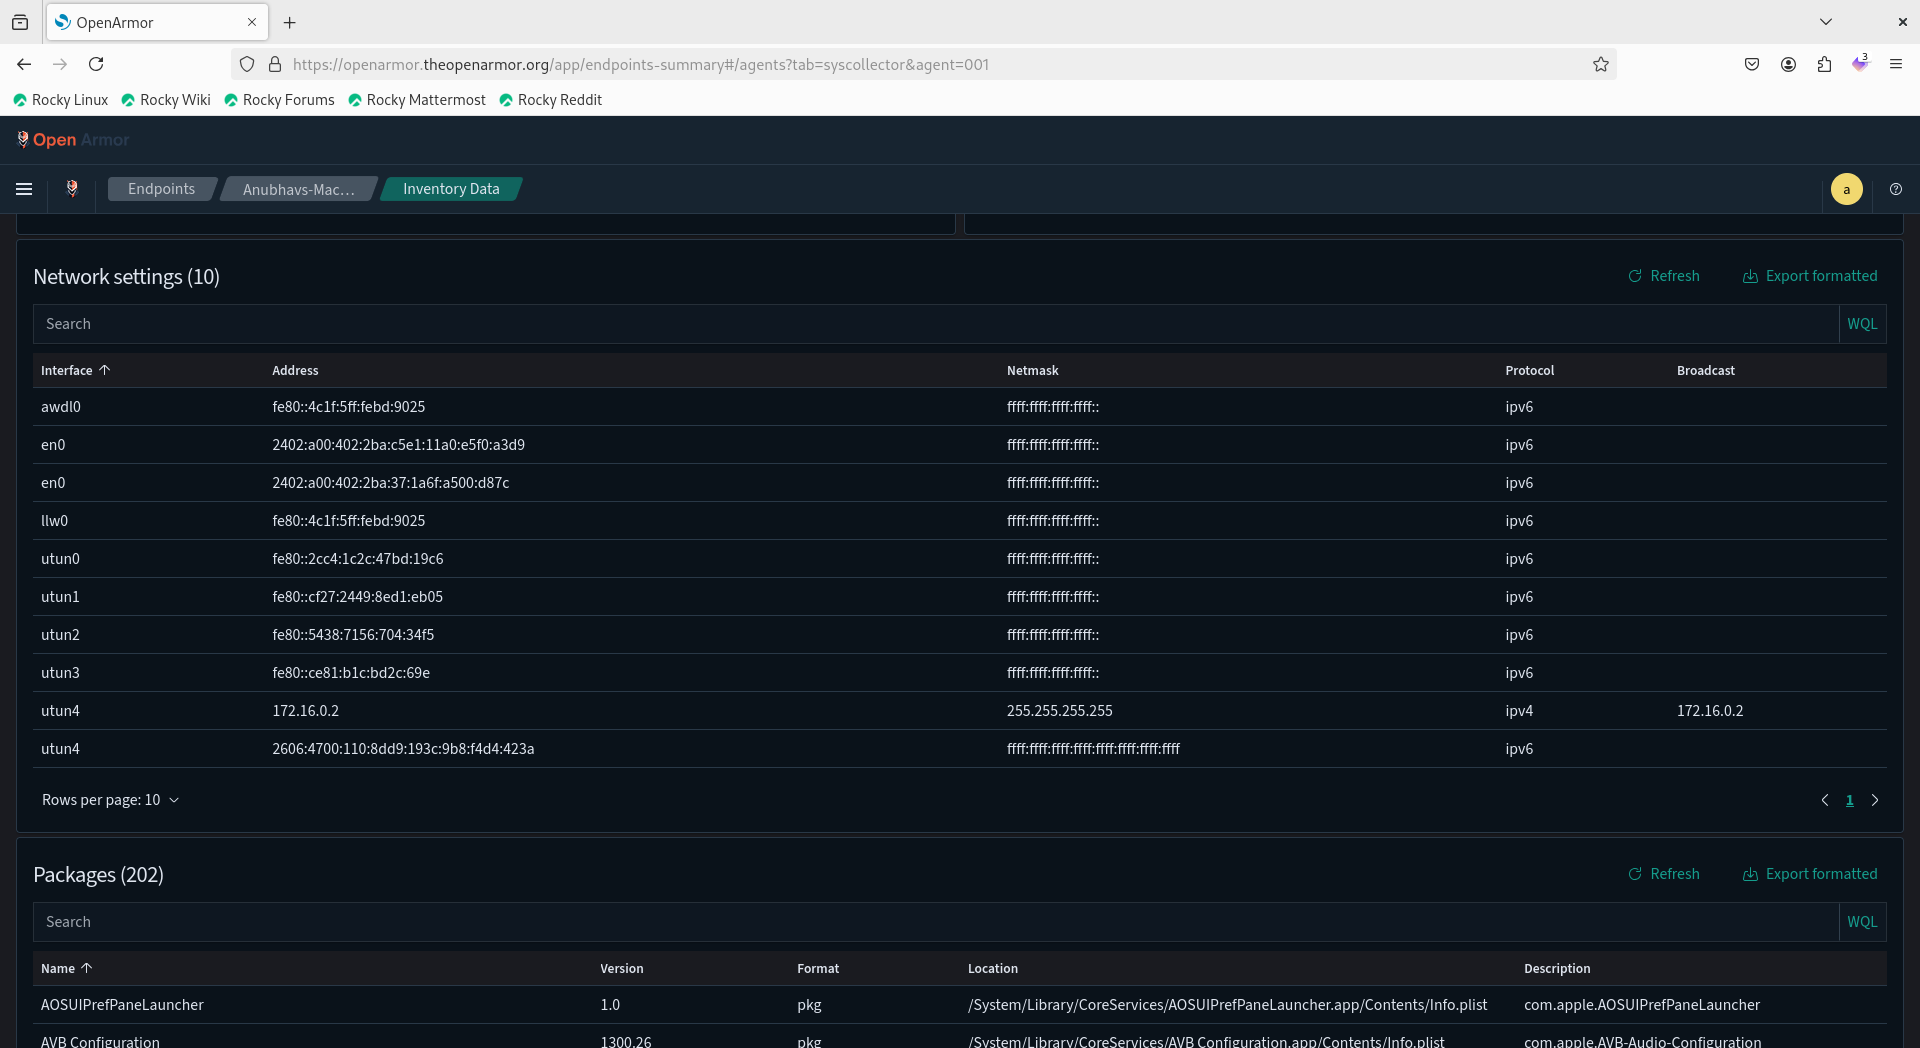
\includegraphics[width=0.7\textwidth]{openarmor-agent/7.png}
    \caption{Load Testing Scenario}
    \label{fig:load-testing}
\end{figure}

\subsection{Latency Testing}
\begin{enumerate}
    \item Measure round-trip time for agent-server communications.
    \item Test latency under various network conditions.
    \item Verify real-time alert capabilities.
\end{enumerate}

\subsection{Reliability Testing}
\begin{enumerate}
    \item Simulate network interruptions between agent and server.
    \item Test agent behavior during server unavailability.
    \item Verify data integrity and synchronization after reconnection.
\end{enumerate}

\section{Integration Testing}
\subsection{SIEM Integration}
\begin{enumerate}
    \item Verify agent data flow to SIEM system.
    \item Test SIEM alert generation based on agent data.
    \item Check SIEM dashboard for agent status and events.
\end{enumerate}

\begin{figure}[h]
    \centering
    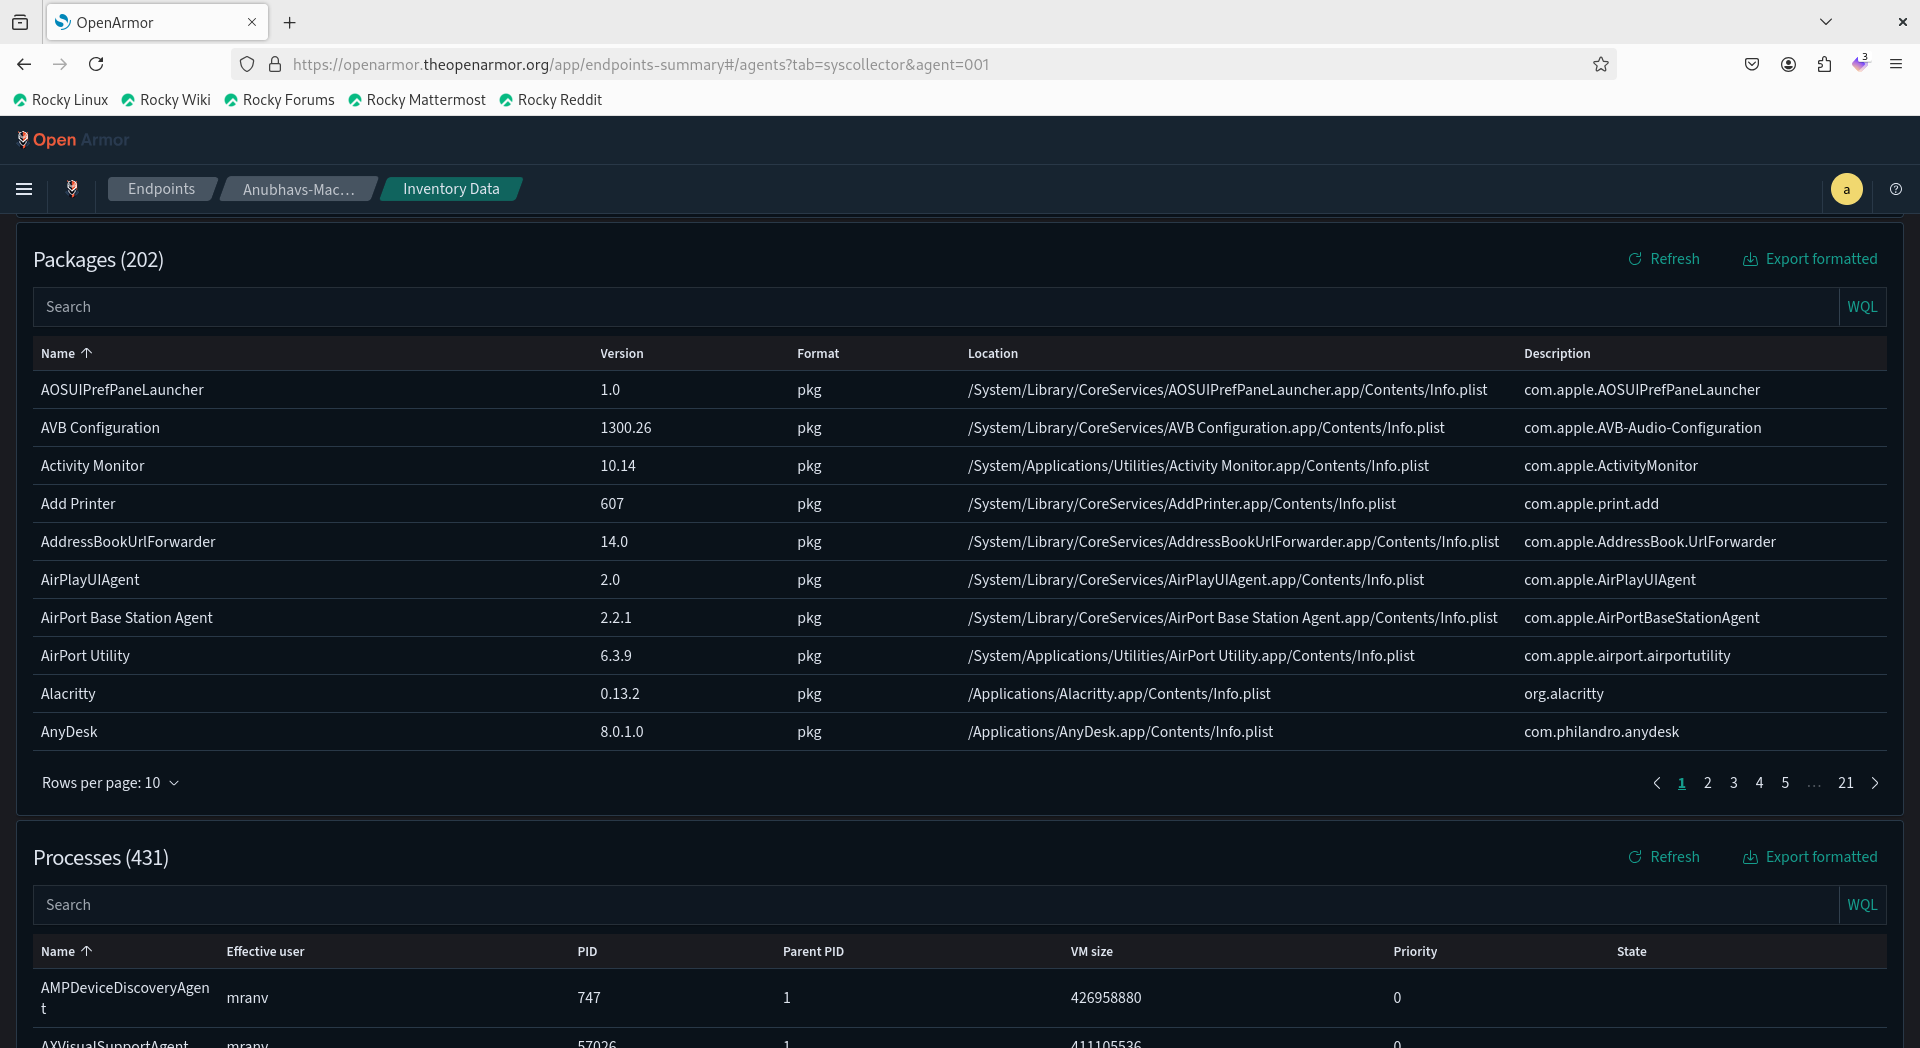
\includegraphics[width=0.8\textwidth]{openarmor-agent/8.png}
    \caption{SIEM Integration Architecture}
    \label{fig:siem-integration}
\end{figure}

\subsection{API Testing}
\begin{enumerate}
    \item Test RESTful API endpoints for agent management.
    \item Verify API authentication and rate limiting.
    \item Validate API responses for various agent operations.
\end{enumerate}

\section{User Acceptance Testing}
\subsection{Dashboard Functionality}
\begin{enumerate}
    \item Verify agent status display on OpenArmor dashboard.
    \item Test filtering and searching capabilities for agent data.
    \item Validate real-time updates of agent information.
\end{enumerate}

\subsection{Reporting}
\begin{enumerate}
    \item Generate reports on agent status and events.
    \item Verify accuracy of agent data in reports.
    \item Test scheduled and on-demand report generation.
\end{enumerate}

\begin{figure}[h]
    \centering
    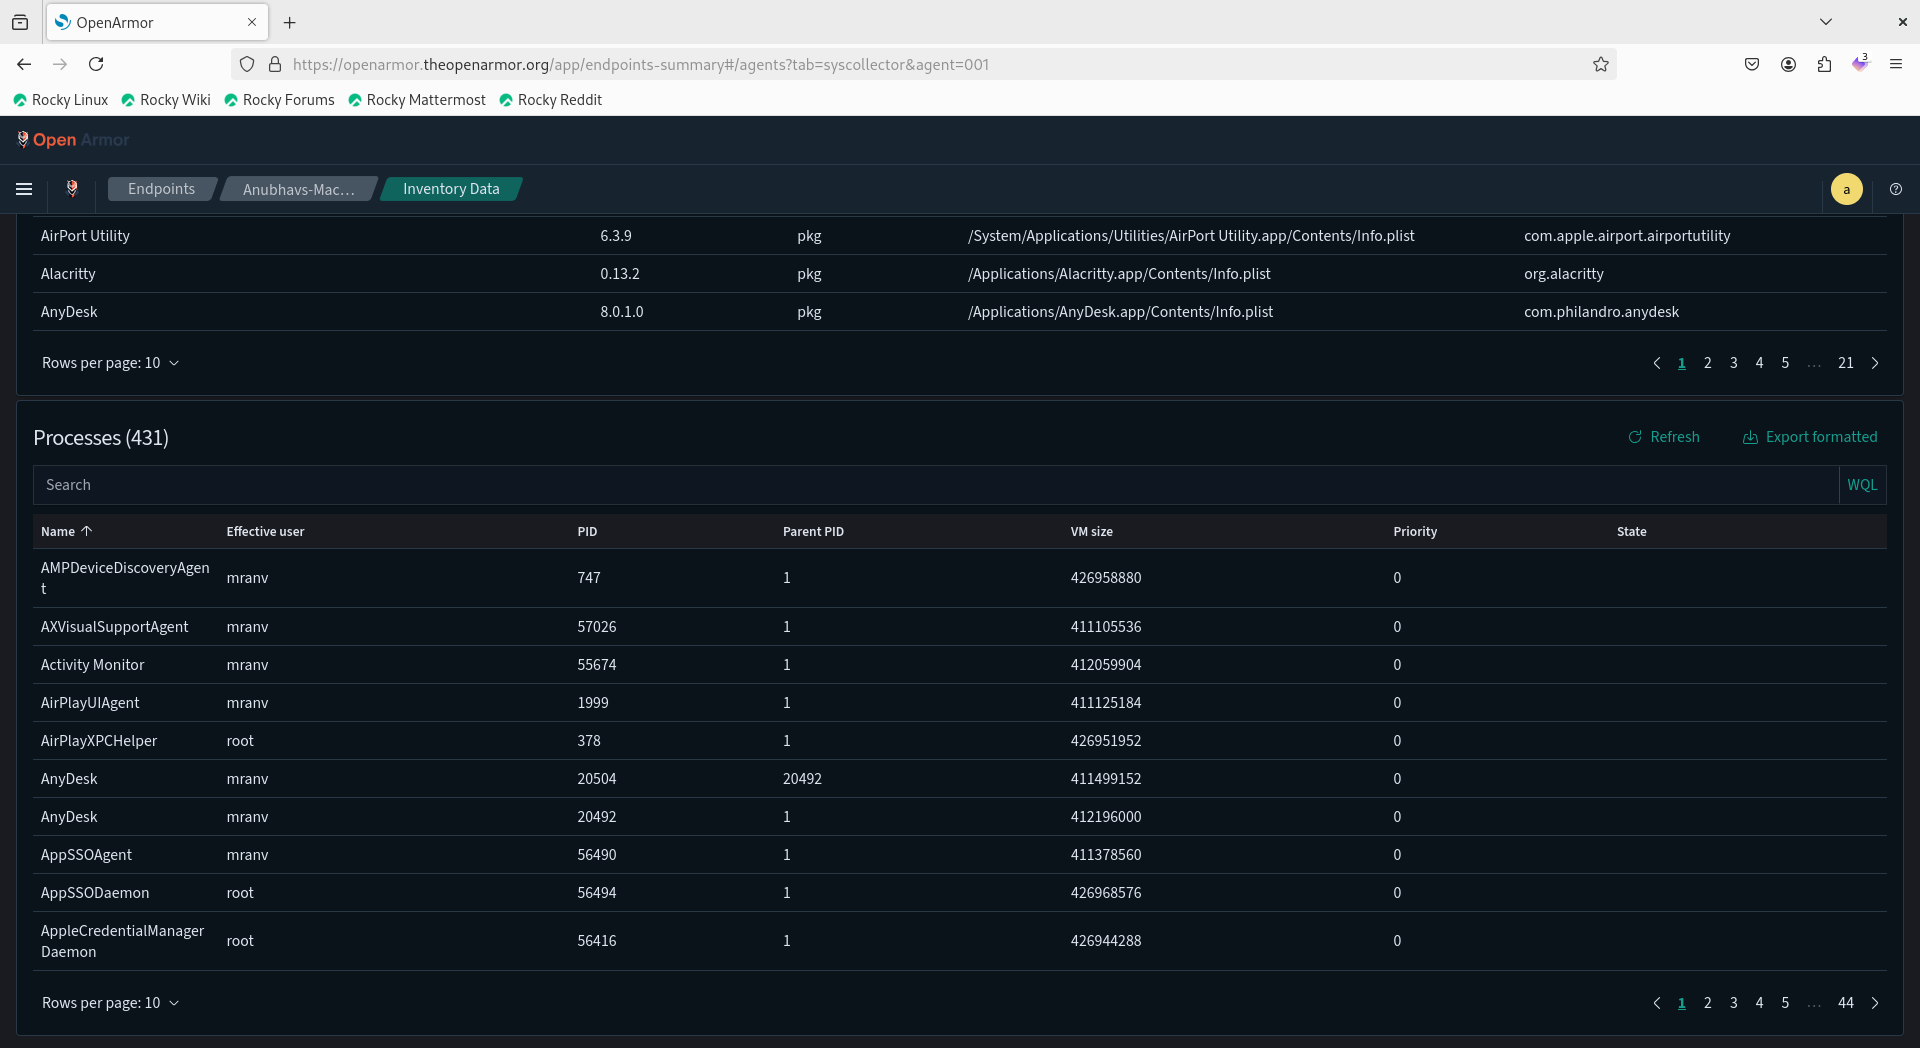
\includegraphics[width=0.7\textwidth]{openarmor-agent/9.png}
    \caption{Sample OpenArmor Dashboard and Reporting Interface}
    \label{fig:dashboard-reporting}
\end{figure}

\section{Conclusion}
This testing documentation provides a comprehensive guide for verifying the OpenArmor agent-server communication. By following these procedures and utilizing the illustrated test scenarios, testers can ensure the reliability, security, and performance of the OpenArmor system. Regular execution of these tests will help maintain the integrity of the agent-server interaction as the system evolves.
\chapter{Conclusion}

OpenArmor represents a significant leap forward in cybersecurity technology, leveraging advanced logging techniques, artificial intelligence, and seamless integration with established security tools to provide a comprehensive and intelligent security solution. As we conclude this project, it's important to reflect on the key achievements, challenges, and future implications of OpenArmor.

\section{Key Achievements}

\begin{itemize}
    \item \textbf{Advanced Logging Capabilities}: By utilizing eBPF technology, OpenArmor has achieved unprecedented visibility into system activities with minimal performance impact. This kernel-level logging provides a depth of insight that traditional logging methods cannot match.
    
    \item \textbf{Seamless Integration}: The successful integration of Wazuh, OSquery, and Sysmon demonstrates OpenArmor's ability to leverage and enhance existing security tools, providing a unified and powerful security platform.
    
    \item \textbf{AI-Driven Analysis}: The implementation of machine learning and artificial intelligence for log processing and threat detection positions OpenArmor at the forefront of proactive cybersecurity measures. These capabilities enable the system to identify complex attack patterns and anomalies that might elude traditional rule-based systems.
    
    \item \textbf{Standardization and Interoperability}: By adopting the OCSF standard, OpenArmor ensures seamless data integration and interoperability with a wide range of security tools and platforms, enhancing its value in diverse IT environments.
    
    \item \textbf{Real-Time Threat Detection}: The combination of advanced logging, AI analysis, and integration with threat intelligence feeds enables OpenArmor to provide real-time threat detection and response capabilities, significantly reducing the time to detect and mitigate potential security incidents.
\end{itemize}

\section{Challenges and Considerations}

While OpenArmor offers powerful capabilities, it's important to acknowledge the challenges associated with implementing and maintaining such an advanced system:

\begin{itemize}
    \item \textbf{Data Volume and Management}: The comprehensive logging capabilities of OpenArmor generate vast amounts of data. Efficient storage, processing, and analysis of this data require robust infrastructure and careful resource management.
    
    \item \textbf{Complexity}: The integration of multiple technologies and the use of advanced AI techniques increase the overall complexity of the system. This complexity necessitates a high level of expertise for proper deployment, configuration, and maintenance.
    
    \item \textbf{False Positives}: Despite advanced AI capabilities, the risk of false positives remains a concern. Continuous tuning and refinement of detection algorithms are necessary to maintain accuracy while minimizing false alarms.
    
    \item \textbf{Privacy and Compliance}: The depth of logging and analysis performed by OpenArmor raises important privacy considerations. Ensuring compliance with data protection regulations and maintaining user privacy requires careful planning and implementation of data governance policies.
    
    \item \textbf{Evolving Threat Landscape}: As cyber threats continue to evolve, OpenArmor must continuously adapt and improve its detection capabilities. This requires ongoing research, development, and updates to maintain effectiveness against new and emerging threats.
\end{itemize}

\section{Future Implications and Potential Impact}

OpenArmor represents a significant step forward in the field of cybersecurity, with potential far-reaching implications:

\begin{itemize}
    \item \textbf{Paradigm Shift in Threat Detection}: By combining advanced logging with AI-driven analysis, OpenArmor has the potential to shift the cybersecurity paradigm from reactive to proactive threat detection, potentially revolutionizing how organizations approach security.
    
    \item \textbf{Enhanced Incident Response}: The real-time capabilities and comprehensive visibility provided by OpenArmor can significantly improve incident response times and effectiveness, potentially reducing the impact of security breaches.
    
    \item \textbf{Ecosystem Development}: As an open and extensible platform, OpenArmor could foster the development of a rich ecosystem of plugins, integrations, and complementary tools, further enhancing its capabilities and adaptability to diverse security needs.
    
    \item \textbf{Cybersecurity Research}: The wealth of data and advanced analysis capabilities offered by OpenArmor could provide valuable insights for cybersecurity research, potentially leading to new discoveries in threat detection and prevention strategies.
    
    \item \textbf{Industry Standards}: OpenArmor's adoption of OCSF and its integration capabilities could contribute to the broader adoption of standardization in cybersecurity, promoting greater interoperability and collaboration within the industry.
\end{itemize}

\section{Closing Thoughts}

OpenArmor stands as a testament to the power of integrating advanced technologies with established security practices. While it presents challenges in implementation and management, the potential benefits in terms of enhanced threat detection, reduced response times, and improved overall security posture are substantial.

As cyber threats continue to evolve in sophistication and scale, solutions like OpenArmor will play a crucial role in empowering organizations to stay ahead of potential security risks. The project not only addresses current cybersecurity needs but also lays a foundation for future advancements in the field.

The success of OpenArmor will ultimately depend on its ability to deliver tangible security improvements while addressing the challenges of complexity, data management, and evolving threats. With continued development, refinement, and adaptation, OpenArmor has the potential to significantly enhance the cybersecurity capabilities of organizations across various sectors, contributing to a more secure digital ecosystem for all.
\chapter{Future Work}

As OpenArmor continues to evolve, several key areas have been identified for future development and enhancement. These improvements aim to expand the system's capabilities, increase its adaptability to diverse environments, and maintain its position at the forefront of intelligent cybersecurity solutions.

\section{Expand Platform Support}
\begin{itemize}
    \item \textbf{Windows Integration}: Develop eBPF-like capabilities for Windows using technologies like ETW (Event Tracing for Windows) or eBPF for Windows.
    \item \textbf{MacOS Support}: Explore integration with macOS's Endpoint Security Framework for comprehensive logging.
    \item \textbf{Cloud-Native Implementations}: 
    \begin{itemize}
        \item Develop cloud-specific agents for major providers (AWS, Azure, GCP).
        \item Implement serverless architectures for improved scalability.
        \item Create Kubernetes operators for seamless deployment in container environments.
    \end{itemize}
\end{itemize}

\section{Enhance Data Collection and Integration}
\begin{itemize}
    \item \textbf{Expand Data Sources}:
    \begin{itemize}
        \item Integrate with cloud service provider logs (CloudTrail, Azure Monitor).
        \item Incorporate IoT device logs and telemetry data.
        \item Develop plugins for popular application and database logs.
    \end{itemize}
    \item \textbf{Advanced Network Telemetry}: Implement deep packet inspection and NetFlow analysis capabilities.
    \item \textbf{Third-Party Integrations}: Develop connectors for popular SIEM, SOAR, and threat intelligence platforms.
\end{itemize}

\section{Advanced AI and Machine Learning Capabilities}
\begin{itemize}
    \item \textbf{Federated Learning}: Implement privacy-preserving federated learning techniques to improve models across multiple deployments.
    \item \textbf{Explainable AI}: Develop techniques to provide clear explanations for AI-driven alerts and decisions.
    \item \textbf{Transfer Learning}: Explore transfer learning approaches to adapt models quickly to new environments.
    \item \textbf{Reinforcement Learning}: Implement RL algorithms for adaptive threat response strategies.
\end{itemize}

\section{Enhanced eBPF Capabilities}
\begin{itemize}
    \item \textbf{Custom eBPF Programs}: Develop an interface for users to write and deploy custom eBPF programs.
    \item \textbf{eBPF-Driven Microservices}: Explore using eBPF for secure and efficient microservices communication.
    \item \textbf{Hardware Offloading}: Investigate eBPF hardware offloading techniques for improved performance.
\end{itemize}

\section{Compliance and Regulatory Frameworks}
\begin{itemize}
    \item \textbf{Automated Compliance Reporting}: Develop modules for automatic generation of compliance reports (PCI DSS, HIPAA, GDPR, etc.).
    \item \textbf{Policy Enforcement}: Implement AI-driven policy enforcement mechanisms based on compliance requirements.
    \item \textbf{Data Sovereignty}: Develop features to ensure data locality and sovereignty compliance.
\end{itemize}

\section{Advanced Threat Detection and Response}
\begin{itemize}
    \item \textbf{Cyber Deception Integration}:
    \begin{itemize}
        \item Implement intelligent honeypots and honeytokens.
        \item Develop deception-aware ML models for improved threat detection.
    \end{itemize}
    \item \textbf{Threat Hunting Automation}: Create AI-driven tools for proactive threat hunting.
    \item \textbf{Advanced Persistent Threat (APT) Detection}: Develop specialized models for detecting long-term, sophisticated attacks.
\end{itemize}

\section{User Experience and Visualization}
\begin{itemize}
    \item \textbf{3D Visualization}: Implement 3D network and threat visualizations for intuitive understanding of complex security landscapes.
    \item \textbf{Natural Language Interfaces}: Develop NLP-based interfaces for querying security data and initiating actions.
    \item \textbf{Augmented Reality Integration}: Explore AR applications for physical security monitoring and incident response.
\end{itemize}

\section{Performance and Scalability}
\begin{itemize}
    \item \textbf{Distributed Processing}: Implement advanced distributed processing techniques for handling massive data volumes.
    \item \textbf{Edge Computing}: Develop edge-based processing capabilities for real-time analysis in IoT environments.
    \item \textbf{Quantum-Resistant Cryptography}: Research and implement quantum-resistant algorithms for future-proofing secure communications.
\end{itemize}

\section{Incident Response and Orchestration}
\begin{itemize}
    \item \textbf{Automated Playbooks}: Develop AI-driven, adaptive incident response playbooks.
    \item \textbf{Cross-Platform Orchestration}: Implement seamless orchestration across on-premises, cloud, and hybrid environments.
    \item \textbf{Collaborative Response}: Create features for multi-team, multi-organization collaborative incident response.
\end{itemize}

\section{Continuous Learning and Improvement}
\begin{itemize}
    \item \textbf{Automated Model Updates}: Implement continuous learning pipelines for real-time model updates.
    \item \textbf{Adversarial Training}: Develop adversarial training techniques to improve model robustness.
    \item \textbf{Community-Driven Intelligence}: Create a platform for sharing anonymized threat intelligence among OpenArmor users.
\end{itemize}

\section{Research Initiatives}
\begin{itemize}
    \item \textbf{AI Ethics in Cybersecurity}: Research ethical implications of AI-driven security decisions.
    \item \textbf{Quantum Computing Applications}: Explore potential applications of quantum computing in cybersecurity.
    \item \textbf{Bio-Inspired Security Models}: Investigate security models inspired by biological immune systems.
\end{itemize}

\section{Conclusion}
The future work outlined for OpenArmor represents a comprehensive roadmap for enhancing its capabilities, expanding its reach, and ensuring its continued relevance in the ever-evolving cybersecurity landscape. By focusing on these areas, OpenArmor aims to push the boundaries of what's possible in intelligent, adaptive cybersecurity solutions, providing organizations with increasingly sophisticated tools to defend against emerging threats.

As the project moves forward, priorities may shift based on technological advancements, emerging threats, and user feedback. The OpenArmor team remains committed to ongoing research, development, and innovation to maintain the system's position as a cutting-edge, comprehensive cybersecurity platform.

% Bibliography
\cleardoublepage
\phantomsection
\addcontentsline{toc}{chapter}{References}
\bibliographystyle{unsrtnat}
\bibliography{references}

\end{document}